\documentclass[runningheads]{llncs}

\usepackage{graphicx}
% Used for displaying a sample figure. If possible, figure files should
% be included in EPS format.
%
% If you use the hyperref package, please uncomment the following line
% to display URLs in blue roman font according to Springer's eBook style:
% \renewcommand\UrlFont{\color{blue}\rmfamily}

\usepackage{amssymb}
\usepackage{mathtools}
\usepackage[ruled,vlined,linesnumbered]{algorithm2e}
\usepackage[capitalise]{cleveref}
\usepackage{tikz}

\crefname{enumii}{Condition}{Conditions}

\begin{document}

%\title{Contribution Title\thanks{Supported by organization x.}}
\title{Weighted Model Counting Without Parameter Variables}

%\titlerunning{Abbreviated paper title}
% If the paper title is too long for the running head, you can set
% an abbreviated paper title here

%\author{First Author\inst{1}\orcidID{0000-1111-2222-3333} \and
%Second Author\inst{2,3}\orcidID{1111-2222-3333-4444} \and
%Third Author\inst{3}\orcidID{2222--3333-4444-5555}}

%\authorrunning{F. Author et al.}
% First names are abbreviated in the running head.
% If there are more than two authors, 'et al.' is used.

%\institute{Princeton University, Princeton NJ 08544, USA \and
%Springer Heidelberg, Tiergartenstr. 17, 69121 Heidelberg, Germany
%\email{lncs@springer.com}\\
%\url{http://www.springer.com/gp/computer-science/lncs} \and
%ABC Institute, Rupert-Karls-University Heidelberg, Heidelberg, Germany\\
%\email{\{abc,lncs\}@uni-heidelberg.de}}

\maketitle              % typeset the header of the contribution

\begin{abstract}
  The abstract should briefly summarize the contents of the paper in
  150--250 words.

  \keywords{First keyword  \and Second keyword \and Another keyword.}
\end{abstract}

\section{Introduction}

\section{Pseudo-Boolean Functions}

\paragraph{Notation.} For any propositional formula $\phi$ over a set of
variables $X$ and $p, q \in \mathbb{R}$, let $[\phi]^p_q\colon 2^X \to
\mathbb{R}$ be a pseudo-Boolean function defined as
\[
  [\phi]^p_q(Y) \coloneqq
  \begin{cases}
    p & \text{if } Y \models \phi \\
    q & \text{otherwise}
  \end{cases}
\]
for any $Y \subseteq X$.

\begin{definition}[Operations] \label{def:operations}
  Let $f, g\colon 2^X \to \mathbb{R}$ be pseudo-Boolean functions, $x, y \in X$,
  $Y = \{y_i\}_{i=1}^n \subseteq X$, and $r \in \mathbb{R}$. Operations such as
  addition and multiplication are defined pointwise as
  \[
    (f+g)(Y) \coloneqq f(Y)+g(Y), \quad \text{and} \quad (f \cdot g)(Y)
    \coloneqq f(Y) \cdot g(Y).
  \]
  Note that this means that binary operations on pseudo-Boolean functions
  inherit properties such as associativity and commutativity. By not
  distinguishing between a real number and a pseudo-Boolean function that always
  returns that number, we can use the same definitions to define \emph{scalar}
  operations as
  \[
    (r+f)(Y) = r+f(Y), \quad \text{and} \quad (r \cdot f)(Y) = r \cdot f(Y).
  \]

  \emph{Restrictions} $f|_{x=0}, f|_{x=1}\colon 2^X \to \mathbb{R}$ of $f$ are
  defined as
  \[
    f|_{x=0}(Y) \coloneqq f(Y \setminus \{x\}), \quad \text{and} \quad
    f|_{x=1}(Y) \coloneqq f(Y \cup \{x\})
  \]
  for all $Y \subseteq X$.

  \emph{Projection} $\exists_x$ is an endomorphism $\exists_x\colon
  \mathbb{R}^{2^X} \to \mathbb{R}^{2^X}$ defined as
  \[
    \exists_xf \coloneqq f|_{x=1} + f|_{x=0}.
  \]
  Since projection is commutative (i.e., $\exists_x\exists_yf =
  \exists_y\exists_xf$) \cite{DBLP:conf/aaai/DudekPV20,DBLP:conf/cp/DudekPV20},
  we can define $\exists_Y\colon \mathbb{R}^{2^X} \to \mathbb{R}^{2^X}$ as
  $\exists_Y \coloneqq \exists_{y_1}\exists_{y_2}\dots\exists_{y_n}$. Throughout
  the paper, projection is assumed to have the lowest precedence (e.g.,
  $\exists_x fg = \exists_x (fg)$).
\end{definition}

NOTE: We list some properties of the operations on pseudo-Boolean functions
discussed in this section that can be conveniently represented using our syntax.
The proofs of all these properties follow directly from the definitions.

\begin{proposition}[Basic Properties] \label{prop:basic}
  For any propositional formulas $\phi$ and $\psi$, and $a, b, c, d \in
  \mathbb{R}$,
  \begin{itemize}
  \item $[\phi]^a_b = [\neg \phi]^b_a$;
  \item $c + [\phi]^a_b = [\phi]^{a+c}_{b+c}$;
  \item $c \cdot [\phi]^a_b = [\phi]^{ac}_{bc}$;
  \item $[\phi]^a_b \cdot [\phi]^c_d = [\phi]^{ac}_{bd}$;
  \item $[\phi]^1_0 \cdot [\psi]_0^1 = [\phi \land \psi]_0^1$.
  \end{itemize}
  And for any pair of pseudo-Boolean functions $f, g \colon 2^X \to \mathbb{R}$
  and $x \in  X$, $(fg)|_{x=i} = f|_{x=i} \cdot g|_{x=i}$ for $i = 0, 1$.
\end{proposition}

\paragraph{References.}
\begin{itemize}
\item Related work without publicly available implementations:
  \begin{itemize}
  \item direct compilation to SDDs \cite{DBLP:conf/ecsqaru/ChoiKD13}
  \item direct compilation to PSDDs, also eliminating parameter variables (a thesis)
  \item maybe two more papers
  \end{itemize}
\end{itemize}

\paragraph{Notes.}
\begin{itemize}
\item Weights on literals other than the positive literals that correspond to
  variables in $X_P$ are redundant as they either are equal to one or duplicate
  an already-defined weight.
\item Mention that formulas, clauses, and models are all treated as sets.
\end{itemize}

\section{Weighted Model Counting}

NOTE: Our definition of WMC is largely based on the standard definition
\cite{DBLP:journals/ai/ChaviraD08}, but explicitly partitions variables into
indicator and parameter variables.

\begin{definition}[WMC Instance]
  A \emph{WMC instance} is a tuple $(\phi, X_I, X_P, w)$, where $X_I$ is
  the set of indicator variables, $X_P$ is the set of parameter variables (with
  $X_I \cap X_P = \emptyset$), $\phi$ is a propositional formula in CNF over
  $X_I \cup X_P$, and $w\colon X_I \cup X_P \cup \{\neg x \mid x \in X_I \cup
  X_P\} \to \mathbb{R}$ is the weight function. The \emph{answer} of the
  instance is $\sum_{Y \models \phi} \prod_{Y \models l} w(l)$.
\end{definition}

\begin{remark}
  Encodings such as \texttt{cd05} and \texttt{cd06} are \emph{not} WMC
  encodings. Instead, they encode Bayesian network inference into instances of
  the \emph{minimum-cardinality} WMC problem, where the answer is defined to be
  $\sum_{Y \models \phi\text{, }|Y| = k} \prod_{Y \models l}
  w(l)$, where $k = \min_{Y \models \phi\text{, }Y \ne \emptyset}
  |Y|$, if $k$ exists, otherwise the answer is zero. This additional
  condition on model cardinality becomes necessary because these encodings
  eliminate clauses of the form $p \Rightarrow i$, where $p \in X_P$ is a
  parameter variable, and $i \in X_I$ is an indicator variable. Nonetheless, our
  transformation algorithm still works on such encodings, although the
  experimental results are discouraging because they use approximately twice as
  many indicator variables. For instance, each binary variable of a Bayesian
  network is encoded using two indicator variables while one would suffice.
\end{remark}

\begin{definition}[PBP Instance] \label{def:new_wmc}
  A \emph{pseudo-Boolean projection} (PBP) instance is a tuple $(F, X, \omega)$,
  where $X$ is the set of variables, $F$ is a set of pseudo-Boolean functions
  $2^X \to \mathbb{R}$, and $\omega \in \mathbb{R}$ is the scaling factor. The
  \emph{answer} of the instance is $\omega \cdot \left(\exists_X\prod_{f \in
      F}f\right)(\emptyset)$.
\end{definition}

NOTE: The constant is inspired by the \texttt{bklm16}
\cite{DBLP:conf/ecai/BartKLM16} encoding.

\section{Parameter Variable Elimination}

\paragraph{Notes.}
\begin{itemize}
\item Let $X_P$ be the set of parameter variable and $X_I$ be the set of
  indicator variables.
\item Parameter variables are either taken from the LMAP file (for encodings
  produced by Ace) or assumed to be the variables that have both weights equal
  to 1.
\item If a parameter variable in a clause is `negated', we can ignore the
  clause. We assume that there are no clauses with more than one instance of
  parameter variables.
\item The second \textbf{foreach} loop can be performed in constant time by
  representing $\phi'$ as a list and assuming that the two 'clauses' are
  adjacent in that list (and incorporating it into the first loop).
\item The $d$ map is constructed in $\mathcal{O}(|X_P|\log|X_P|)$ time (we want
  to use a data structure based on binary search trees rather than hashing).
\item \texttt{rename} can be implemented in $\mathcal{O}(\log |X_P|)$ time.
\item This may look like preprocessing, but all the transformations are local
  and thus can be incorporated into an encoding algorithm with no slowdown. In
  fact, if anything, the resulting algorithm would be slightly faster, as it
  would have less data to output.
\end{itemize}

\begin{algorithm}[t]
  \caption{WMC instance transformation}
  \label{alg:transformation}
  \SetKwFunction{rename}{rename}
  \SetKwProg{Fn}{Function}{:}{}
  \KwData{WMC instance $(\phi, X_I, X_P, w)$}
  \KwResult{PBP instance $(F, X, \omega)$}
  $F \gets \emptyset$\;
  $\omega \gets 1$\;
  let $d\colon X_P \to \mathbb{N}$ be defined as $p \mapsto |\{ o \in X_P \mid o
  \le p \}|$\;
  \ForEach{clause $c \in \phi$\label{line:foreach1start}}{
    \uIf{$c \cap X_P = \{ p \}$ for some $p$ \textnormal{\textbf{and}} $w(p) \ne
      1$}{
      \uIf{$|c| = 1$}{$\omega \gets \omega \times w(p)$\;}
      \Else{
        $F \gets F \cup \left\{ \left[ \bigwedge_{l \in c \setminus
              \{p\}} \neg l \right]^{w(p)}_1 \right\}$\;
      }
    }
    \ElseIf{$\{p \mid \neg p \in c\} \cap X_P  = \emptyset$}{
      $F \gets F \cup \{ [c]^1_0 \}$\; \label{line:foreach1end}
    }
  }
  \ForEach{indicator variable $v \in X_I$ \label{line:foreach2start}}{
    \If{$\{[v]_1^p, [\neg v]_1^q\} \subseteq F$ for some $p$ and $q$}{
      $F \gets F \setminus \{ [v]_1^p, [\neg v]_1^q \} \cup \{ [v]_q^p
      \}$\; \label{line:foreach2end}
    }
  }
  replace every variable $v$ in $F$ with $\rename{$v$}$\;
  \Return{$(F, X_I, \omega)$}\;
  \Fn{\rename{$v$}}{
    $S \gets \{u \in X_P \mid u \le v\}$\;
    \lIf{$S = \emptyset$}{\Return{$v$}}
    \Return{$v - d(\max S)$}\;
  }
\end{algorithm}

\subsection{Proof of Correctness}

\begin{theorem}[Early Projection
  \cite{DBLP:conf/aaai/DudekPV20,DBLP:conf/cp/DudekPV20},
  verbatim] \label{thm:early}
  Let $X$ and $Y$ be sets of variables. For all functions $f\colon 2^X \to
  \mathbb{R}$ and $g\colon 2^Y \to \mathbb{R}$, if $x \in X \setminus Y$, then
  $\exists_x (f \cdot g) = (\exists_x f) \cdot g$.
\end{theorem}

\begin{lemma} \label{lemma:sum}
  For any pseudo-Boolean function $f\colon 2^X \to \mathbb{R}$,
  \[
    (\exists_X f)(\emptyset) = \sum_{Y \subseteq X} f(Y).
  \]
\end{lemma}
\begin{proof}
  For base case, let $X = \{x\}$. Then
  \[
    (\exists_xf)(\emptyset) = (f|_{x=1} + f|_{x=0})(\emptyset) =
    f|_{x=1}(\emptyset) + f|_{x=0}(\emptyset) = \sum_{Y \subseteq \{x\}} f(Y).
  \]
  This easily extends to $|X| > 1$ by the definition of projection on sets of
  variables.
\end{proof}

% NOTE: mention that this is similar (but not equal) to the DPMC/ADDMC result
\begin{proposition} \label{prop:equivalence}
  Let $(\phi, X_I, X_P, w)$ be a WMC instance. Then
  \begin{equation}
  \left(\left\{[c]_0^1 \;\middle|\; c \in \phi\right\} \cup \left\{[x]_{w(\neg
        x)}^{w(x)} \;\middle|\; x \in X_I \cup X_P\right\}, X_I \cup X_P,
    1\right) \label{eq:new_wmc}
  \end{equation}
  is a PBP instance with the same answer.
\end{proposition}
\begin{proof}
  The answer of \cref{eq:new_wmc} is
  \begin{align*}
    \left(\exists_{X_I \cup X_P} \left(\prod_{c \in \phi} [c]_0^1\right) \prod_{x \in X_I \cup X_P} [x]_{w(\neg x)}^{w(x)} \right)(\emptyset) &= \sum_{Y \subseteq X_I \cup X_P} \left(\left(\prod_{c \in \phi} [c]_0^1 \right) \prod_{x \in X_I \cup X_P} [x]_{w(\neg x)}^{w(x)}\right)(Y) \\
&= \sum_{Y \subseteq X_I \cup X_P} \underbrace{\left(\prod_{c \in \phi} [c]_0^1\right)}_f(Y) \underbrace{\left(\prod_{x \in X_I \cup X_P} [x]_{w(\neg x)}^{w(x)}\right)}_g(Y)
  \end{align*}
  by \cref{lemma:sum}. Note that
  \[
    f(Y) =
    \begin{cases}
      1 & \text{if } Y \models \phi, \\
      0 & \text{otherwise},
    \end{cases}
    \quad
    \text{and}
    \quad
    g(Y) = \prod_{Y \models l} w(l),
  \]
  which means that
  \[
    \sum_{Y \subseteq X_I \cup X_P} f(Y)g(Y) = \sum_{Y \models \phi} \prod_{Y
      \models l} w(l)
  \]
  as required.
\end{proof}

\begin{theorem}[Correctness]
  \Cref{alg:transformation}, when given a WMC instance $(\phi, X_I, X_P,
  w)$, returns PBP instance with the same answer, provided the following
  conditions are satisfied:
  \begin{enumerate}
  \item for all indicator variables $i \in X_I$, $w(i) = w(\neg i) = 1$,
  \item and either
    \begin{enumerate}
    \item for all parameter variables $p \in X_P$, there is a non-empty family
      of literals $(l_i)_{i=1}^n$ such that \label{condition:d02}
      \begin{enumerate}
      \item $w(\neg p) = 1$,
      \item $l_i \in X_I$ or $\neg l_i \in X_I$ for all $i = 1, \dots, n$,
        \label{condition:equivalence1}
      \item and $\{ c \in \phi \mid p \in c \text{ or } \neg p \in c \} =
        \left\{p \lor \bigvee_{i=1}^n \neg l_i \right\} \cup \{ l_i \lor \neg p
        \mid i = 1, \dots, n \}$; \label{condition:equivalence2}
      \end{enumerate}
    \item or for all parameter variables $p \in X_P$, \label{condition:bklm16}
      \begin{enumerate}
      \item $w(p) + w(\neg p) = 1$,
      \item for any clause $c \in \phi$, $|c \cap X_P| \le 1$,
      \item there is no clause $c \in \phi$ such that $\neg p \in c$,
      \item if $\{ p \} \in \phi$, then there is no clause $c \in \phi$ such
        that $c \ne \{ p \}$ and $p \in c$, \label{cond:just_parameter}
        % 'prime implicants are logically disjoint'
      \item and for any $c, d \in \phi$ such that $c \ne d$, $p \in c$ and $p
        \in d$, $\bigwedge_{l \in c \setminus \{ p \}} \neg l \land \bigwedge_{l
          \in d \setminus \{ p \}} \neg l$ is false. \label{cond:disjoint}
      \end{enumerate}
    \end{enumerate}
  \end{enumerate}
\end{theorem}
\begin{proof}
  By \cref{prop:equivalence},
  \begin{equation}
    \left(\left\{[c]_0^1 \;\middle|\; c \in \phi\right\} \cup \left\{[x]_{w(\neg
          x)}^{w(x)} \;\middle|\; x \in X_I \cup X_P\right\}, X_I \cup X_P,
      1\right) \label{eq:new_wmc2}
  \end{equation}
  is a PBP instance with the same answer as the given WMC instance. By
  \cref{def:new_wmc}, its answer is
  \begin{equation} \label{eq:answer}
    \left(\exists_{X_I \cup X_P} \left( \prod_{c \in \phi} [c]_0^1 \right) \prod_{x \in X_I \cup X_P} [x]_{w(\neg x)}^{w(x)} \right)(\emptyset)
  \end{equation}
  Since both \cref{condition:d02,condition:bklm16} ensure that each clause in
  $\phi$ has at most one parameter variable, we can partition $\phi$ into
  $\phi_* \coloneqq \{c \in \phi \mid \mathtt{Vars}(c) \cap X_P = \emptyset \}$
  and $\phi_p \coloneqq \{ c \in \phi \mid \mathtt{Vars}(c) \cap X_P = \{ p \}
  \}$ for all $p \in X_P$. We can then use \cref{thm:early} to reorder
  \eqref{eq:answer} into
  \[
    \left(\exists_{X_I} \left( \prod_{x \in X_I} [x]_{w(\neg x)}^{w(x)} \right)
      \left( \prod_{c \in \phi_*} [c]_0^1 \right) \prod_{p \in X_P} \exists_p
      [p]_{w(\neg p)}^{w(p)} \prod_{c \in \phi_p} [c]_0^1 \right)(\emptyset).
  \]

  Let us first consider how the unfinished WMC instance $(F, X_I, \omega)$ after
  the loop on \crefrange{line:foreach1start}{line:foreach1end} differs from
  \eqref{eq:new_wmc2}. Note that \cref{alg:transformation} leaves each $c \in
  \phi_*$ unchanged, i.e., adds $[c]_0^1$ to $F$. We can then fix an arbitrary
  $p \in X_P$ and let $F_p$ be the set of functions added to $F$ as a
  replacement of $\phi_p$. It is sufficient to show that
  \begin{equation} \label{eq:to_show}
    \omega \prod_{f \in F_p} f = \exists_p [p]_{w(\neg p)}^{w(p)} \prod_{c \in \phi_p} [c]_0^1.
  \end{equation}
  Note that under \cref{condition:d02},
  \[
    \bigwedge_{c \in \phi_p} c \equiv p \Leftrightarrow \bigwedge_{i=1}^n l_i
  \]
  for some family of indicator variable literals $(l_i)_{i=1}^n$. Thus,
  \[
    \exists_p [p]_{w(\neg p)}^{w(p)} \prod_{c \in \phi_p} [c]_0^1 = \exists_p
    [p]_1^{w(p)} \left[ p \Leftrightarrow \bigwedge_{i=1}^n l_i \right]_0^1.
  \]
  If $w(p) = 1$, then
  \begin{equation} \label{eq:bigsums}
    \exists_p [p]_1^{w(p)} \left[ p \Leftrightarrow \bigwedge_{i=1}^n l_i
    \right]_0^1 = \exists_p \left[ p \Leftrightarrow \bigwedge_{i=1}^n l_i
    \right]_0^1 = \left.\left[ p \Leftrightarrow \bigwedge_{i=1}^n l_i
    \right]_0^1\right|_{p=1} + \left.\left[ p \Leftrightarrow \bigwedge_{i=1}^n
      l_i \right]_0^1\right|_{p=0}.
  \end{equation}
  Since for any input, $\bigwedge_{i=1}^n l_i$ is either true or false, exactly
  one of the two summands in \cref{eq:bigsums} will be equal to one, and the
  other will be equal to zero, and so
  \[
    \left.\left[ p \Leftrightarrow \bigwedge_{i=1}^n l_i
      \right]_0^1\right|_{p=1} + \left.\left[ p \Leftrightarrow \bigwedge_{i=1}^n
        l_i \right]_0^1\right|_{p=0} = 1,
  \]
  where $1$ is a pseudo-Boolean function that always returns one. On the other
  side of \cref{eq:to_show}, since $F_p = \emptyset$, and $\omega$ is unchanged,
  we get $\omega\prod_{f \in F_p} f = 1$, and so \cref{eq:to_show} is satisfied
  under \cref{condition:d02} when $w(p) = 1$.

  If $w(p) \ne 1$, then
  \[
    F_p = \left\{ \left[ \bigwedge_{i = 1}^n l_i \right]_1^{w(p)} \right\},
  \]
  and $\omega = 1$, and so we want to show that
  \[
    \left[ \bigwedge_{i = 1}^n l_i \right]_1^{w(p)} = \exists_p [p]_1^{w(p)}
    \left[ p \Leftrightarrow \bigwedge_{i=1}^n l_i \right]_0^1,
  \]
  and indeed
  \begin{align*}
    \exists_p [p]_1^{w(p)} \left[ p \Leftrightarrow \bigwedge_{i=1}^n l_i \right]_0^1 &= \left.\left( [p]_1^{w(p)} \left[ p \Leftrightarrow \bigwedge_{i=1}^n l_i \right]_0^1 \right)\right|_{p=1} + \left.\left([p]_1^{w(p)} \left[ p \Leftrightarrow \bigwedge_{i=1}^n l_i \right]_0^1 \right)\right|_{p=0} \\
                                                                                      &= w(p) \cdot \left[ \bigwedge_{i=1}^n l_i \right]_0^1 + \left[ \bigwedge_{i=1}^n l_i \right]_1^0 = \left[ \bigwedge_{i=1}^n l_i \right]_1^{w(p)}.
  \end{align*}
  This finishes the proof of the correctness of the first `foreach' loop under
  \cref{condition:d02}.

  Now let us assume \cref{condition:bklm16}. We still want to prove
  \cref{eq:to_show}. If $w(p) = 1$, then $F_p = \emptyset$, and $\omega = 1$,
  and so the left-hand side of \cref{eq:to_show} is equal to one. Then the
  right-hand side is
  \[
    \exists_p [p]_0^1 \prod_{c \in \phi_p} [c]_0^1 = \exists_p \left[ p \land
      \bigwedge_{c \in \phi_p} c \right]_0^1 = \exists_p [p]_0^1 = 0 + 1 = 1
  \]
  since $p \in c$ for every clause $c \in \phi_p$.

  If $w(p) \ne 1$, and $\{ p \} \in \phi_p$, then, by
  \cref{cond:just_parameter}, $\phi_p = \{ \{ p \} \}$, and
  \cref{alg:transformation} produces $F_p = \emptyset$ and $\omega = w(p)$, and
  so
  \[
    \exists_p [p]_{w(\neg p)}^{w(p)} [p]_0^1 = \exists_p [p]^{w(p)}_0 = w(p) =
    \omega \prod_{f \in F_p} f.
  \]
  The only remaining case is when $w(p) \ne 1$ and $\{ p \} \not \in \phi_p$.
  Then $\omega = 1$, and
  \[
    F_p = \left\{ \left[\bigwedge_{l \in c \setminus \{ p \}} \neg
        l\right]_1^{w(p)} \;\middle|\; c \in \phi_p \right\},
  \]
  so need to show that
  \[
    \prod_{c \in \phi_p} \left[\bigwedge_{l \in c \setminus \{ p \}} \neg
      l\right]_1^{w(p)} = \exists_p [p]_{1-w(p)}^{w(p)} \prod_{c \in \phi_p}
    [c]_0^1.
  \]
  We can rearrange the right-hand side as
  \begin{align*}
    \exists_p [p]_{1-w(p)}^{w(p)} \prod_{c \in \phi_p} [c]_0^1 &= \exists_p [p]_{1-w(p)}^{w(p)} \left[\bigwedge_{c \in \phi_p} c\right]_0^1 = \exists_p [p]_{1-w(p)}^{w(p)} \left[ p \lor \bigwedge_{c \in \phi_p} c \setminus \{ p \} \right]_0^1 \\
                                                               &= w(p) + (1-w(p)) \left[ \bigwedge_{c \in \phi_p} c \setminus \{ p \} \right]_0^1 = w(p) + \left[ \bigwedge_{c \in \phi_p} c \setminus \{ p \} \right]_0^{1-w(p)} \\
                                                               &= \left[ \bigwedge_{c \in \phi_p} c \setminus \{ p \} \right]_{w(p)}^1 = \left[ \neg \bigwedge_{c \in \phi_p} c \setminus \{ p \} \right]_1^{w(p)} = \left[ \bigvee_{c \in \phi_p} \neg(c \setminus \{ p \}) \right]_1^{w(p)} \\
                                                               &= \left[ \bigvee_{c \in \phi_p} \neg \bigvee_{l \in c \setminus \{ p \}} l \right]_1^{w(p)} = \left[ \bigvee_{c \in \phi_p} \bigwedge_{l \in c \setminus \{ p \}} \neg l \right]_1^{w(p)}.
  \end{align*}
   By \cref{cond:disjoint}, $\bigwedge_{l \in c \setminus \{ p \}} \neg l$ can
   be true for at most one $c \in \phi_p$, and so
   \[
     \left[ \bigvee_{c \in \phi_p} \bigwedge_{l \in c \setminus \{ p \}} \neg l
     \right]_1^{w(p)} = \prod_{c \in \phi_p} \left[ \bigwedge_{l \in c \setminus
         \{ p \}} \neg l \right]_1^{w(p)}
   \]
   which is exactly what we needed to show. This ends the proof that the
   first loop of \cref{alg:transformation} preserves the answer under both
   \cref{condition:d02} and \cref{condition:bklm16}. Finally, the loop on
   \crefrange{line:foreach2start}{line:foreach2end} of \cref{alg:transformation}
   replaces $[v]_1^p[\neg v]_1^q$ with $[v]_q^p$ (for some $v \in X_I$ and $p, q
   \in \mathbb{R}$), but, of course,
   \[
     [v]_1^p[\neg v]_1^q = [v]_1^p[v]_q^1 = [v]_q^p,
   \]
   i.e., the answer is unchanged.
\end{proof}

\section{Experimental Results}

\paragraph{Notes.}
\begin{itemize}
\item Apparently, the \textsc{DPMC} paper \cite{DBLP:conf/cp/DudekPV20} already
  shows that taking the first offered decomposition tree is best.
\item Processors:
  \begin{itemize}
  \item Intel(R) Xeon(R) Gold 6138 CPU @ 2.00GHz
  \item Intel(R) Xeon(R) CPU E5-2630 v3 @ 2.40GHz
  \item Intel(R) Xeon(R) CPU E7-4820 v2 @ 2.00GHz
  \end{itemize}
\end{itemize}

\begin{figure}[t]
  \centering
  % Created by tikzDevice version 0.12.3 on 2020-08-01 17:20:52
% !TEX encoding = UTF-8 Unicode
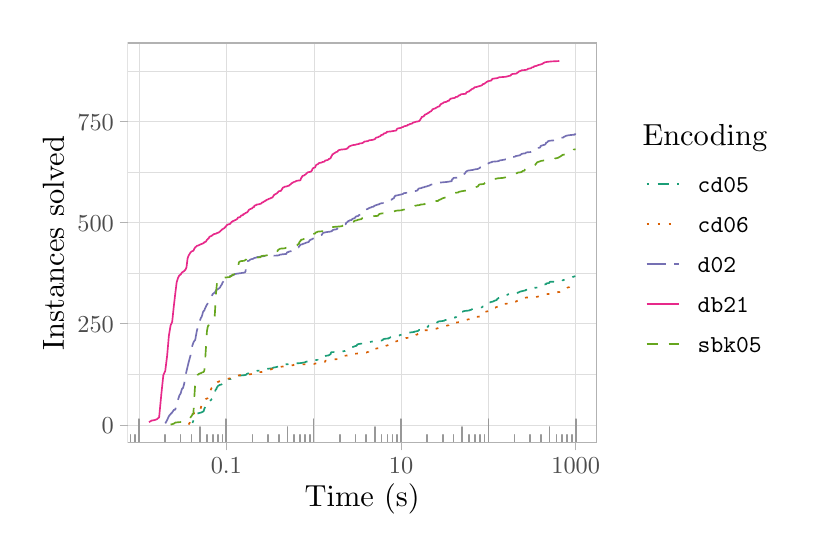
\begin{tikzpicture}[x=1pt,y=1pt]
\definecolor{fillColor}{RGB}{255,255,255}
\path[use as bounding box,fill=fillColor,fill opacity=0.00] (0,0) rectangle (278.24,180.67);
\begin{scope}
\path[clip] (  0.00,  0.00) rectangle (278.24,180.67);
\definecolor{drawColor}{RGB}{255,255,255}
\definecolor{fillColor}{RGB}{255,255,255}

\path[draw=drawColor,line width= 0.6pt,line join=round,line cap=round,fill=fillColor] (  0.00,  0.00) rectangle (278.24,180.68);
\end{scope}
\begin{scope}
\path[clip] ( 36.11, 30.69) rectangle (205.68,175.17);
\definecolor{fillColor}{RGB}{255,255,255}

\path[fill=fillColor] ( 36.11, 30.69) rectangle (205.68,175.17);
\definecolor{drawColor}{gray}{0.87}

\path[draw=drawColor,line width= 0.1pt,line join=round] ( 36.11, 55.37) --
	(205.68, 55.37);

\path[draw=drawColor,line width= 0.1pt,line join=round] ( 36.11, 91.90) --
	(205.68, 91.90);

\path[draw=drawColor,line width= 0.1pt,line join=round] ( 36.11,128.43) --
	(205.68,128.43);

\path[draw=drawColor,line width= 0.1pt,line join=round] ( 36.11,164.95) --
	(205.68,164.95);

\path[draw=drawColor,line width= 0.1pt,line join=round] ( 40.22, 30.69) --
	( 40.22,175.17);

\path[draw=drawColor,line width= 0.1pt,line join=round] (103.34, 30.69) --
	(103.34,175.17);

\path[draw=drawColor,line width= 0.1pt,line join=round] (166.47, 30.69) --
	(166.47,175.17);

\path[draw=drawColor,line width= 0.3pt,line join=round] ( 36.11, 37.11) --
	(205.68, 37.11);

\path[draw=drawColor,line width= 0.3pt,line join=round] ( 36.11, 73.64) --
	(205.68, 73.64);

\path[draw=drawColor,line width= 0.3pt,line join=round] ( 36.11,110.16) --
	(205.68,110.16);

\path[draw=drawColor,line width= 0.3pt,line join=round] ( 36.11,146.69) --
	(205.68,146.69);

\path[draw=drawColor,line width= 0.3pt,line join=round] ( 71.78, 30.69) --
	( 71.78,175.17);

\path[draw=drawColor,line width= 0.3pt,line join=round] (134.91, 30.69) --
	(134.91,175.17);

\path[draw=drawColor,line width= 0.3pt,line join=round] (198.03, 30.69) --
	(198.03,175.17);
\definecolor{drawColor}{RGB}{27,158,119}

\path[draw=drawColor,line width= 0.6pt,dash pattern=on 1pt off 3pt on 4pt off 3pt ,line join=round] ( 59.56, 37.84) --
	( 59.89, 38.71) --
	( 60.22, 39.74) --
	( 60.53, 40.47) --
	( 60.84, 40.91) --
	( 61.14, 41.20) --
	( 62.82, 41.64) --
	( 63.59, 42.08) --
	( 63.84, 42.95) --
	( 64.08, 43.54) --
	( 64.32, 44.41) --
	( 64.55, 44.85) --
	( 64.78, 45.14) --
	( 65.01, 45.29) --
	( 65.23, 45.44) --
	( 65.45, 45.58) --
	( 65.88, 45.87) --
	( 66.09, 46.02) --
	( 66.29, 46.17) --
	( 66.50, 46.46) --
	( 66.89, 46.75) --
	( 67.09, 47.34) --
	( 67.28, 47.63) --
	( 67.47, 48.07) --
	( 67.66, 48.80) --
	( 67.84, 49.67) --
	( 68.02, 49.97) --
	( 68.20, 50.11) --
	( 68.38, 50.70) --
	( 68.55, 50.84) --
	( 68.73, 51.13) --
	( 68.90, 51.28) --
	( 69.39, 51.57) --
	( 70.03, 51.72) --
	( 70.19, 51.86) --
	( 70.34, 52.01) --
	( 70.49, 52.16) --
	( 70.64, 52.60) --
	( 70.79, 52.74) --
	( 70.94, 53.03) --
	( 71.08, 53.18) --
	( 71.37, 53.33) --
	( 71.92, 53.47) --
	( 72.32, 53.62) --
	( 73.46, 53.76) --
	( 73.58, 53.91) --
	( 73.82, 54.20) --
	( 74.73, 54.35) --
	( 74.84, 54.49) --
	( 75.38, 54.64) --
	( 76.00, 54.79) --
	( 76.20, 54.93) --
	( 78.14, 55.08) --
	( 78.89, 55.23) --
	( 79.06, 55.37) --
	( 79.14, 55.52) --
	( 79.38, 55.66) --
	( 79.84, 55.81) --
	( 80.80, 55.96) --
	( 81.01, 56.10) --
	( 81.56, 56.25) --
	( 82.15, 56.39) --
	( 82.40, 56.54) --
	( 82.90, 56.69) --
	( 84.51, 56.83) --
	( 85.55, 56.98) --
	( 85.60, 57.12) --
	( 86.14, 57.27) --
	( 86.75, 57.42) --
	( 88.27, 57.56) --
	( 88.56, 57.71) --
	( 88.92, 57.86) --
	( 89.68, 58.00) --
	( 90.33, 58.15) --
	( 91.26, 58.29) --
	( 92.25, 58.44) --
	( 92.67, 58.59) --
	( 92.82, 58.73) --
	( 92.88, 58.88) --
	( 93.23, 59.02) --
	( 95.54, 59.17) --
	( 95.78, 59.32) --
	( 98.51, 59.46) --
	( 99.60, 59.61) --
	(100.18, 59.75) --
	(100.44, 59.90) --
	(100.97, 60.05) --
	(102.70, 60.19) --
	(102.77, 60.34) --
	(103.18, 60.49) --
	(104.73, 60.63) --
	(104.84, 60.78) --
	(104.86, 60.92) --
	(105.61, 61.07) --
	(105.71, 61.22) --
	(105.76, 61.36) --
	(106.49, 61.65) --
	(106.71, 61.80) --
	(107.11, 61.95) --
	(107.66, 62.09) --
	(108.70, 62.24) --
	(108.94, 62.38) --
	(109.14, 62.53) --
	(109.44, 62.68) --
	(109.53, 62.82) --
	(109.55, 62.97) --
	(109.56, 63.12) --
	(109.61, 63.26) --
	(109.79, 63.41) --
	(113.34, 63.55) --
	(113.86, 63.70) --
	(114.65, 63.85) --
	(114.85, 63.99) --
	(114.96, 64.14) --
	(115.67, 64.28) --
	(115.88, 64.43) --
	(115.93, 64.58) --
	(116.05, 64.72) --
	(116.59, 64.87) --
	(116.80, 65.01) --
	(117.01, 65.16) --
	(117.54, 65.31) --
	(117.99, 65.45) --
	(118.33, 65.60) --
	(118.91, 65.75) --
	(118.95, 65.89) --
	(119.00, 66.04) --
	(119.07, 66.18) --
	(119.49, 66.33) --
	(120.39, 66.48) --
	(122.58, 66.62) --
	(123.52, 66.77) --
	(123.65, 66.91) --
	(123.88, 67.06) --
	(124.05, 67.21) --
	(125.63, 67.35) --
	(125.97, 67.50) --
	(127.90, 67.64) --
	(128.29, 67.79) --
	(128.40, 67.94) --
	(128.51, 68.08) --
	(128.93, 68.23) --
	(130.47, 68.38) --
	(130.56, 68.52) --
	(130.91, 68.67) --
	(131.06, 68.81) --
	(132.13, 68.96) --
	(132.68, 69.11) --
	(132.88, 69.25) --
	(134.33, 69.40) --
	(134.38, 69.54) --
	(134.92, 69.69) --
	(135.51, 69.84) --
	(135.83, 69.98) --
	(136.08, 70.13) --
	(136.75, 70.27) --
	(137.17, 70.42) --
	(138.61, 70.57) --
	(139.62, 70.71) --
	(139.84, 70.86) --
	(140.77, 71.01) --
	(141.17, 71.15) --
	(141.26, 71.30) --
	(141.42, 71.44) --
	(143.11, 71.59) --
	(143.19, 71.74) --
	(143.46, 71.88) --
	(144.14, 72.03) --
	(144.34, 72.17) --
	(144.37, 72.32) --
	(144.48, 72.47) --
	(144.58, 72.61) --
	(144.79, 72.76) --
	(144.81, 72.90) --
	(144.95, 73.05) --
	(145.24, 73.20) --
	(145.47, 73.34) --
	(145.92, 73.49) --
	(147.23, 73.64) --
	(147.44, 73.78) --
	(147.46, 73.93) --
	(147.72, 74.07) --
	(148.22, 74.22) --
	(148.27, 74.37) --
	(148.30, 74.51) --
	(149.81, 74.66) --
	(150.57, 74.80) --
	(150.66, 74.95) --
	(151.33, 75.10) --
	(151.51, 75.24) --
	(151.72, 75.39) --
	(152.00, 75.53) --
	(152.11, 75.68) --
	(152.77, 75.83) --
	(154.61, 75.97) --
	(154.83, 76.12) --
	(154.90, 76.27) --
	(154.95, 76.41) --
	(155.00, 76.56) --
	(155.20, 76.70) --
	(155.26, 76.85) --
	(155.28, 77.00) --
	(155.81, 77.14) --
	(155.83, 77.29) --
	(155.95, 77.43) --
	(156.19, 77.58) --
	(156.23, 77.73) --
	(156.33, 77.87) --
	(157.14, 78.02) --
	(157.39, 78.16) --
	(158.01, 78.31) --
	(159.50, 78.46) --
	(159.73, 78.60) --
	(160.29, 78.75) --
	(160.47, 78.90) --
	(161.11, 79.04) --
	(161.73, 79.19) --
	(162.65, 79.33) --
	(163.23, 79.48) --
	(164.16, 79.63) --
	(164.29, 79.77) --
	(164.53, 79.92) --
	(165.13, 80.06) --
	(165.72, 80.21) --
	(165.75, 80.36) --
	(165.77, 80.50) --
	(166.15, 80.65) --
	(166.22, 80.79) --
	(166.27, 80.94) --
	(166.35, 81.09) --
	(166.35, 81.23) --
	(167.05, 81.38) --
	(167.35, 81.53) --
	(168.04, 81.67) --
	(168.37, 81.82) --
	(168.61, 81.96) --
	(169.05, 82.11) --
	(169.51, 82.26) --
	(169.52, 82.40) --
	(169.62, 82.55) --
	(169.80, 82.69) --
	(169.96, 82.84) --
	(170.15, 82.99) --
	(170.56, 83.13) --
	(170.65, 83.28) --
	(170.96, 83.42) --
	(171.94, 83.57) --
	(172.12, 83.72) --
	(172.36, 83.86) --
	(172.47, 84.01) --
	(173.42, 84.16) --
	(173.44, 84.30) --
	(175.96, 84.45) --
	(176.63, 84.59) --
	(176.97, 84.74) --
	(176.99, 84.89) --
	(177.55, 85.03) --
	(177.57, 85.18) --
	(178.08, 85.32) --
	(178.68, 85.47) --
	(179.32, 85.62) --
	(179.91, 85.76) --
	(180.02, 85.91) --
	(181.06, 86.05) --
	(181.14, 86.20) --
	(181.21, 86.35) --
	(182.87, 86.49) --
	(182.94, 86.64) --
	(184.41, 86.79) --
	(184.74, 86.93) --
	(184.93, 87.08) --
	(185.23, 87.22) --
	(185.27, 87.37) --
	(185.96, 87.52) --
	(186.07, 87.66) --
	(186.19, 87.81) --
	(187.31, 87.95) --
	(187.35, 88.10) --
	(187.37, 88.25) --
	(188.44, 88.39) --
	(188.53, 88.54) --
	(188.55, 88.68) --
	(188.68, 88.83) --
	(192.45, 88.98) --
	(193.20, 89.12) --
	(193.28, 89.27) --
	(193.38, 89.42) --
	(193.89, 89.56) --
	(194.14, 89.71) --
	(194.52, 89.85) --
	(195.52, 90.00) --
	(195.91, 90.15) --
	(196.52, 90.29) --
	(196.72, 90.44) --
	(196.95, 90.58) --
	(197.43, 90.73) --
	(197.91, 90.88);
\definecolor{drawColor}{RGB}{217,95,2}

\path[draw=drawColor,line width= 0.6pt,dash pattern=on 1pt off 3pt ,line join=round] ( 58.16, 37.25) --
	( 58.52, 37.84) --
	( 58.88, 39.59) --
	( 59.22, 40.47) --
	( 59.56, 41.05) --
	( 60.22, 41.34) --
	( 61.14, 41.49) --
	( 61.43, 41.78) --
	( 62.01, 41.93) --
	( 62.28, 42.08) --
	( 62.55, 43.24) --
	( 62.82, 44.27) --
	( 63.08, 44.85) --
	( 63.34, 45.44) --
	( 63.84, 45.87) --
	( 64.08, 46.02) --
	( 64.32, 46.46) --
	( 65.01, 46.75) --
	( 65.23, 46.90) --
	( 65.45, 47.34) --
	( 65.67, 47.77) --
	( 65.88, 48.65) --
	( 66.09, 49.53) --
	( 66.29, 50.11) --
	( 66.50, 50.55) --
	( 66.70, 50.84) --
	( 66.89, 51.43) --
	( 67.09, 51.57) --
	( 67.28, 51.72) --
	( 67.47, 51.86) --
	( 67.84, 52.01) --
	( 68.02, 52.16) --
	( 68.38, 52.30) --
	( 68.55, 52.60) --
	( 69.06, 52.74) --
	( 69.23, 52.89) --
	( 69.56, 53.03) --
	( 69.87, 53.18) --
	( 70.19, 53.33) --
	( 70.94, 53.47) --
	( 71.65, 53.62) --
	( 71.78, 53.76) --
	( 72.97, 53.91) --
	( 73.46, 54.06) --
	( 73.82, 54.20) --
	( 74.28, 54.49) --
	( 74.84, 54.64) --
	( 74.95, 54.79) --
	( 75.49, 54.93) --
	( 76.59, 55.08) --
	( 79.22, 55.23) --
	( 79.84, 55.37) --
	( 81.01, 55.52) --
	( 81.08, 55.66) --
	( 81.15, 55.81) --
	( 82.34, 55.96) --
	( 82.72, 56.10) --
	( 84.56, 56.25) --
	( 85.50, 56.39) --
	( 86.19, 56.54) --
	( 86.47, 56.69) --
	( 87.11, 56.83) --
	( 87.34, 56.98) --
	( 87.73, 57.12) --
	( 88.11, 57.27) --
	( 88.44, 57.42) --
	( 88.72, 57.56) --
	( 90.61, 57.86) --
	( 90.85, 58.00) --
	( 91.55, 58.15) --
	( 92.76, 58.29) --
	( 93.82, 58.44) --
	( 94.85, 58.59) --
	( 96.09, 58.73) --
	( 96.16, 58.88) --
	(100.27, 59.02) --
	(103.56, 59.17) --
	(103.99, 59.32) --
	(104.98, 59.46) --
	(105.40, 59.61) --
	(106.51, 59.75) --
	(107.46, 59.90) --
	(107.47, 60.05) --
	(107.50, 60.19) --
	(107.71, 60.34) --
	(108.64, 60.49) --
	(109.52, 60.63) --
	(110.62, 60.78) --
	(112.04, 60.92) --
	(112.14, 61.07) --
	(112.60, 61.22) --
	(112.83, 61.36) --
	(113.18, 61.51) --
	(113.48, 61.65) --
	(113.88, 61.80) --
	(114.05, 61.95) --
	(114.28, 62.09) --
	(115.62, 62.24) --
	(117.04, 62.38) --
	(117.14, 62.53) --
	(117.17, 62.68) --
	(117.61, 62.82) --
	(120.08, 62.97) --
	(120.83, 63.12) --
	(122.39, 63.26) --
	(122.72, 63.41) --
	(123.16, 63.55) --
	(123.21, 63.70) --
	(123.36, 63.85) --
	(123.36, 63.99) --
	(123.39, 64.14) --
	(123.45, 64.28) --
	(123.90, 64.43) --
	(125.26, 64.58) --
	(126.04, 64.72) --
	(126.78, 64.87) --
	(126.86, 65.01) --
	(126.88, 65.16) --
	(127.97, 65.31) --
	(128.41, 65.45) --
	(129.17, 65.60) --
	(129.56, 65.75) --
	(130.06, 65.89) --
	(130.38, 66.04) --
	(130.54, 66.18) --
	(130.85, 66.33) --
	(130.89, 66.48) --
	(131.15, 66.62) --
	(131.28, 66.77) --
	(132.02, 66.91) --
	(132.22, 67.06) --
	(132.44, 67.21) --
	(133.43, 67.35) --
	(133.58, 67.50) --
	(134.96, 67.64) --
	(135.14, 67.79) --
	(135.24, 67.94) --
	(135.48, 68.08) --
	(135.83, 68.23) --
	(136.36, 68.38) --
	(136.68, 68.52) --
	(138.14, 68.67) --
	(138.61, 68.81) --
	(139.38, 68.96) --
	(139.38, 69.11) --
	(139.57, 69.25) --
	(139.89, 69.40) --
	(140.07, 69.54) --
	(140.31, 69.69) --
	(140.91, 69.84) --
	(140.91, 69.98) --
	(141.45, 70.13) --
	(141.90, 70.27) --
	(142.10, 70.42) --
	(142.92, 70.57) --
	(143.07, 70.71) --
	(143.09, 70.86) --
	(143.28, 71.01) --
	(143.30, 71.15) --
	(143.55, 71.30) --
	(145.67, 71.44) --
	(145.79, 71.59) --
	(146.91, 71.74) --
	(147.53, 71.88) --
	(148.12, 72.03) --
	(148.43, 72.17) --
	(149.21, 72.32) --
	(149.80, 72.47) --
	(149.98, 72.61) --
	(150.56, 72.76) --
	(150.83, 72.90) --
	(151.81, 73.05) --
	(152.13, 73.20) --
	(152.20, 73.34) --
	(152.27, 73.49) --
	(152.29, 73.64) --
	(152.51, 73.78) --
	(153.79, 73.93) --
	(154.57, 74.07) --
	(155.62, 74.22) --
	(156.39, 74.37) --
	(156.92, 74.51) --
	(157.40, 74.66) --
	(157.72, 74.80) --
	(158.16, 74.95) --
	(158.71, 75.10) --
	(159.02, 75.24) --
	(160.09, 75.39) --
	(161.11, 75.53) --
	(161.61, 75.68) --
	(161.61, 75.83) --
	(161.64, 75.97) --
	(161.96, 76.12) --
	(163.07, 76.27) --
	(163.87, 76.41) --
	(164.09, 76.56) --
	(164.16, 76.70) --
	(164.19, 76.85) --
	(164.19, 77.00) --
	(164.27, 77.14) --
	(164.36, 77.29) --
	(164.37, 77.43) --
	(164.74, 77.58) --
	(164.89, 77.73) --
	(165.08, 77.87) --
	(165.27, 78.02) --
	(166.19, 78.16) --
	(166.53, 78.31) --
	(167.14, 78.46) --
	(167.22, 78.60) --
	(167.32, 78.75) --
	(167.41, 78.90) --
	(167.47, 79.04) --
	(167.60, 79.19) --
	(168.37, 79.33) --
	(168.97, 79.48) --
	(169.19, 79.63) --
	(169.60, 79.77) --
	(169.95, 79.92) --
	(170.05, 80.06) --
	(170.07, 80.21) --
	(170.29, 80.36) --
	(170.32, 80.50) --
	(171.11, 80.65) --
	(172.05, 80.79) --
	(173.03, 80.94) --
	(174.96, 81.09) --
	(175.34, 81.23) --
	(175.36, 81.38) --
	(175.59, 81.53) --
	(176.49, 81.67) --
	(176.54, 81.82) --
	(176.94, 81.96) --
	(177.77, 82.11) --
	(178.02, 82.26) --
	(178.10, 82.40) --
	(178.99, 82.55) --
	(179.08, 82.69) --
	(179.24, 82.84) --
	(179.51, 82.99) --
	(179.99, 83.13) --
	(183.14, 83.28) --
	(183.99, 83.42) --
	(184.68, 83.57) --
	(185.02, 83.72) --
	(185.75, 83.86) --
	(186.49, 84.01) --
	(186.80, 84.16) --
	(187.12, 84.30) --
	(188.18, 84.45) --
	(190.60, 84.59) --
	(190.74, 84.74) --
	(190.94, 84.89) --
	(191.10, 85.03) --
	(192.25, 85.18) --
	(192.34, 85.32) --
	(192.58, 85.47) --
	(192.67, 85.62) --
	(193.26, 85.76) --
	(193.55, 85.91) --
	(194.02, 86.05) --
	(194.49, 86.20) --
	(194.66, 86.35) --
	(194.75, 86.49) --
	(194.92, 86.64) --
	(195.22, 86.79) --
	(195.70, 86.93) --
	(195.72, 87.08) --
	(195.89, 87.22) --
	(196.24, 87.37) --
	(196.29, 87.52) --
	(196.68, 87.66);
\definecolor{drawColor}{RGB}{117,112,179}

\path[draw=drawColor,line width= 0.6pt,dash pattern=on 7pt off 3pt ,line join=round] ( 49.72, 37.69) --
	( 50.39, 38.86) --
	( 51.03, 40.32) --
	( 51.64, 41.05) --
	( 52.22, 41.64) --
	( 52.78, 42.51) --
	( 53.32, 42.66) --
	( 53.84, 44.56) --
	( 54.34, 46.31) --
	( 54.82, 47.77) --
	( 55.28, 48.50) --
	( 55.73, 50.11) --
	( 56.17, 50.55) --
	( 56.59, 52.16) --
	( 57.00, 54.93) --
	( 57.39, 56.54) --
	( 57.78, 58.15) --
	( 58.16, 59.75) --
	( 58.52, 61.07) --
	( 58.88, 62.38) --
	( 59.22, 64.87) --
	( 59.56, 65.89) --
	( 59.89, 66.91) --
	( 60.22, 67.50) --
	( 60.53, 67.79) --
	( 60.84, 69.54) --
	( 61.14, 71.15) --
	( 61.43, 72.17) --
	( 61.72, 73.49) --
	( 62.01, 74.07) --
	( 62.28, 74.95) --
	( 62.55, 75.68) --
	( 62.82, 76.12) --
	( 63.08, 76.85) --
	( 63.34, 77.87) --
	( 63.59, 78.31) --
	( 63.84, 78.46) --
	( 64.08, 79.19) --
	( 64.32, 79.63) --
	( 64.55, 80.21) --
	( 65.01, 80.94) --
	( 65.23, 81.38) --
	( 65.45, 81.82) --
	( 65.67, 82.40) --
	( 65.88, 82.84) --
	( 66.09, 83.28) --
	( 66.29, 83.57) --
	( 66.50, 83.86) --
	( 66.70, 84.01) --
	( 66.89, 84.45) --
	( 67.09, 84.59) --
	( 67.28, 84.74) --
	( 67.66, 85.03) --
	( 67.84, 85.32) --
	( 68.02, 85.76) --
	( 68.20, 85.91) --
	( 68.55, 86.05) --
	( 68.73, 86.20) --
	( 69.39, 86.64) --
	( 69.56, 86.93) --
	( 69.72, 87.22) --
	( 69.87, 87.52) --
	( 70.03, 87.66) --
	( 70.19, 87.95) --
	( 70.34, 88.39) --
	( 70.49, 88.68) --
	( 70.64, 88.83) --
	( 70.79, 89.12) --
	( 71.08, 89.27) --
	( 71.22, 89.42) --
	( 71.37, 89.85) --
	( 71.65, 90.00) --
	( 71.78, 90.15) --
	( 71.92, 90.29) --
	( 72.06, 90.44) --
	( 72.45, 90.58) --
	( 72.58, 90.73) --
	( 72.97, 90.88) --
	( 73.34, 91.02) --
	( 73.94, 91.17) --
	( 74.40, 91.31) --
	( 74.62, 91.46) --
	( 74.73, 91.61) --
	( 75.49, 91.75) --
	( 76.49, 91.90) --
	( 78.48, 92.19) --
	( 78.73, 92.63) --
	( 78.81, 93.51) --
	( 78.89, 93.80) --
	( 78.98, 94.68) --
	( 79.06, 95.26) --
	( 79.14, 95.84) --
	( 79.22, 96.14) --
	( 79.30, 96.28) --
	( 79.84, 96.43) --
	( 80.14, 96.57) --
	( 80.22, 96.72) --
	( 80.44, 96.87) --
	( 80.80, 97.01) --
	( 81.49, 97.16) --
	( 81.89, 97.45) --
	( 82.65, 97.60) --
	( 82.84, 97.74) --
	( 83.90, 97.89) --
	( 84.45, 98.04) --
	( 86.33, 98.18) --
	( 90.23, 98.33) --
	( 90.89, 98.47) --
	( 91.09, 98.62) --
	( 92.03, 98.77) --
	( 93.45, 98.91) --
	( 93.54, 99.06) --
	( 93.60, 99.20) --
	( 93.68, 99.35) --
	( 93.73, 99.50) --
	( 94.33, 99.64) --
	( 94.49, 99.79) --
	( 95.47, 99.94) --
	( 95.88,100.08) --
	( 96.14,100.23) --
	( 96.18,100.37) --
	( 96.21,100.52) --
	( 96.32,100.67) --
	( 96.39,100.81) --
	( 96.86,100.96) --
	( 97.21,101.10) --
	( 97.92,101.25) --
	( 97.96,101.54) --
	( 98.18,101.69) --
	( 98.22,101.83) --
	( 98.42,101.98) --
	( 98.46,102.13) --
	( 98.51,102.27) --
	( 99.37,102.42) --
	( 99.53,102.57) --
	(100.03,102.71) --
	(100.41,102.86) --
	(100.71,103.00) --
	(101.28,103.15) --
	(101.65,103.30) --
	(101.67,103.44) --
	(101.75,103.59) --
	(101.78,103.73) --
	(102.02,103.88) --
	(102.14,104.03) --
	(102.71,104.17) --
	(102.84,104.32) --
	(103.10,104.46) --
	(103.52,104.61) --
	(103.56,104.76) --
	(103.82,104.90) --
	(104.18,105.05) --
	(104.65,105.20) --
	(104.75,105.34) --
	(104.92,105.49) --
	(105.22,105.63) --
	(106.18,105.78) --
	(106.45,105.93) --
	(106.46,106.07) --
	(106.51,106.22) --
	(106.59,106.36) --
	(106.79,106.51) --
	(107.32,106.66) --
	(107.97,106.80) --
	(109.12,106.95) --
	(109.80,107.09) --
	(109.95,107.24) --
	(110.13,107.39) --
	(110.22,107.53) --
	(110.65,107.68) --
	(111.64,107.83) --
	(111.78,107.97) --
	(111.95,108.12) --
	(112.27,108.26) --
	(112.36,108.41) --
	(112.47,108.56) --
	(112.69,108.70) --
	(113.03,108.85) --
	(114.03,108.99) --
	(114.08,109.14) --
	(114.37,109.29) --
	(114.57,109.43) --
	(114.79,109.58) --
	(114.97,109.72) --
	(115.02,109.87) --
	(115.04,110.02) --
	(115.06,110.16) --
	(115.34,110.31) --
	(115.59,110.46) --
	(115.77,110.75) --
	(116.16,110.89) --
	(116.35,111.04) --
	(117.07,111.19) --
	(117.12,111.33) --
	(117.28,111.48) --
	(117.45,111.62) --
	(117.98,111.77) --
	(118.20,111.92) --
	(118.36,112.06) --
	(118.39,112.21) --
	(118.53,112.35) --
	(118.78,112.50) --
	(119.53,112.65) --
	(119.57,112.79) --
	(119.71,112.94) --
	(120.24,113.09) --
	(120.43,113.23) --
	(120.58,113.38) --
	(120.81,113.52) --
	(120.97,113.67) --
	(121.10,113.82) --
	(121.14,113.96) --
	(121.40,114.11) --
	(121.75,114.25) --
	(121.90,114.40) --
	(121.92,114.55) --
	(122.03,114.69) --
	(122.04,114.84) --
	(122.28,114.98) --
	(122.73,115.13) --
	(123.10,115.28) --
	(123.21,115.42) --
	(123.55,115.57) --
	(124.13,115.72) --
	(124.25,115.86) --
	(125.09,116.01) --
	(125.12,116.15) --
	(125.21,116.30) --
	(125.70,116.45) --
	(126.00,116.59) --
	(126.50,116.74) --
	(127.06,116.88) --
	(127.13,117.03) --
	(127.65,117.18) --
	(128.70,117.32) --
	(128.88,117.47) --
	(129.48,117.61) --
	(129.52,117.76) --
	(129.82,117.91) --
	(129.97,118.05) --
	(130.10,118.20) --
	(130.58,118.35) --
	(131.41,118.49) --
	(131.72,118.64) --
	(131.73,118.78) --
	(132.11,118.93) --
	(132.37,119.08) --
	(132.41,119.22) --
	(132.42,119.37) --
	(132.49,119.51) --
	(132.72,119.66) --
	(132.72,119.81) --
	(132.75,119.95) --
	(133.66,120.10) --
	(134.25,120.24) --
	(134.93,120.39) --
	(135.48,120.54) --
	(135.77,120.68) --
	(135.79,120.83) --
	(136.82,120.98) --
	(138.98,121.12) --
	(139.04,121.27) --
	(139.29,121.41) --
	(139.48,121.56) --
	(140.44,121.71) --
	(140.86,121.85) --
	(140.91,122.00) --
	(141.03,122.14) --
	(141.08,122.29) --
	(141.19,122.44) --
	(141.46,122.58) --
	(142.34,122.73) --
	(142.44,122.87) --
	(143.30,123.02) --
	(143.50,123.17) --
	(144.24,123.31) --
	(144.60,123.46) --
	(145.17,123.61) --
	(145.40,123.75) --
	(145.59,123.90) --
	(146.20,124.04) --
	(146.25,124.19) --
	(146.60,124.34) --
	(147.98,124.48) --
	(148.31,124.63) --
	(149.79,124.77) --
	(151.46,124.92) --
	(152.37,125.07) --
	(153.22,125.21) --
	(153.24,125.36) --
	(153.25,125.50) --
	(153.31,125.65) --
	(153.37,125.80) --
	(153.51,125.94) --
	(153.74,126.09) --
	(153.76,126.24) --
	(153.92,126.38) --
	(155.79,126.53) --
	(155.99,126.67) --
	(156.04,126.82) --
	(156.04,126.97) --
	(156.06,127.11) --
	(156.08,127.26) --
	(156.62,127.40) --
	(156.85,127.55) --
	(157.50,127.70) --
	(157.82,127.84) --
	(157.99,127.99) --
	(158.09,128.13) --
	(158.18,128.28) --
	(158.30,128.43) --
	(158.32,128.57) --
	(158.55,128.72) --
	(158.76,128.87) --
	(159.03,129.01) --
	(160.11,129.16) --
	(161.06,129.30) --
	(161.46,129.45) --
	(162.59,129.60) --
	(162.89,129.74) --
	(163.16,129.89) --
	(163.42,130.03) --
	(163.50,130.18) --
	(164.13,130.33) --
	(164.20,130.47) --
	(164.21,130.62) --
	(165.03,130.76) --
	(165.20,130.91) --
	(165.51,131.06) --
	(165.65,131.20) --
	(165.73,131.35) --
	(165.97,131.50) --
	(166.64,131.64) --
	(166.66,131.79) --
	(167.17,131.93) --
	(167.70,132.08) --
	(167.82,132.23) --
	(169.68,132.37) --
	(170.34,132.52) --
	(170.38,132.66) --
	(171.34,132.81) --
	(172.16,132.96) --
	(172.76,133.10) --
	(174.66,133.25) --
	(174.70,133.39) --
	(174.80,133.54) --
	(174.87,133.69) --
	(175.14,133.83) --
	(175.66,133.98) --
	(176.26,134.13) --
	(176.37,134.27) --
	(177.25,134.42) --
	(177.92,134.56) --
	(177.99,134.71) --
	(178.29,134.86) --
	(178.40,135.00) --
	(178.89,135.15) --
	(179.91,135.29) --
	(180.01,135.44) --
	(180.14,135.59) --
	(181.73,135.73) --
	(181.96,135.88) --
	(182.22,136.02) --
	(182.93,136.17) --
	(183.17,136.32) --
	(183.41,136.46) --
	(183.58,136.61) --
	(184.30,136.76) --
	(184.33,136.90) --
	(184.47,137.05) --
	(184.50,137.19) --
	(185.12,137.34) --
	(185.22,137.49) --
	(185.26,137.63) --
	(185.32,137.78) --
	(185.34,137.92) --
	(185.80,138.07) --
	(186.21,138.22) --
	(186.89,138.36) --
	(186.98,138.51) --
	(187.10,138.65) --
	(187.27,138.80) --
	(187.27,138.95) --
	(187.31,139.09) --
	(187.68,139.24) --
	(187.91,139.39) --
	(187.92,139.53) --
	(188.12,139.68) --
	(188.71,139.82) --
	(190.50,139.97) --
	(190.82,140.12) --
	(191.62,140.26) --
	(191.66,140.41) --
	(192.27,140.55) --
	(192.48,140.70) --
	(192.66,140.85) --
	(193.59,140.99) --
	(193.66,141.14) --
	(193.94,141.28) --
	(194.26,141.43) --
	(194.47,141.58) --
	(195.06,141.72) --
	(196.16,141.87) --
	(197.75,142.02) --
	(197.84,142.16) --
	(197.88,142.31) --
	(197.96,142.45);
\definecolor{drawColor}{RGB}{231,41,138}

\path[draw=drawColor,line width= 0.6pt,line join=round] ( 43.82, 38.13) --
	( 44.83, 38.71) --
	( 45.78, 38.86) --
	( 46.66, 39.15) --
	( 47.50, 39.88) --
	( 48.28, 48.07) --
	( 49.02, 55.08) --
	( 49.72, 56.69) --
	( 50.39, 62.09) --
	( 51.03, 69.40) --
	( 51.64, 73.05) --
	( 52.22, 74.37) --
	( 52.78, 79.77) --
	( 53.32, 84.45) --
	( 53.84, 88.68) --
	( 54.34, 90.29) --
	( 54.82, 91.17) --
	( 55.28, 91.46) --
	( 55.73, 92.19) --
	( 56.59, 92.78) --
	( 57.00, 93.21) --
	( 57.39, 94.09) --
	( 57.78, 97.31) --
	( 58.16, 98.33) --
	( 58.52, 98.91) --
	( 58.88, 99.50) --
	( 59.22, 99.79) --
	( 59.89,100.08) --
	( 60.22,100.81) --
	( 60.53,101.25) --
	( 60.84,101.54) --
	( 61.14,101.83) --
	( 61.72,101.98) --
	( 62.01,102.13) --
	( 62.28,102.27) --
	( 62.55,102.42) --
	( 63.08,102.57) --
	( 63.34,102.71) --
	( 63.59,102.86) --
	( 63.84,103.15) --
	( 64.32,103.30) --
	( 64.55,103.59) --
	( 64.78,104.03) --
	( 65.01,104.17) --
	( 65.23,104.46) --
	( 65.45,104.61) --
	( 65.67,105.05) --
	( 65.88,105.20) --
	( 66.29,105.34) --
	( 66.50,105.49) --
	( 66.70,105.63) --
	( 67.28,106.07) --
	( 68.02,106.22) --
	( 68.20,106.36) --
	( 68.55,106.51) --
	( 69.06,106.66) --
	( 69.39,106.95) --
	( 69.72,107.24) --
	( 69.87,107.39) --
	( 70.03,107.53) --
	( 70.19,107.68) --
	( 70.34,107.83) --
	( 70.64,107.97) --
	( 71.08,108.26) --
	( 71.22,108.41) --
	( 71.37,108.56) --
	( 71.51,108.70) --
	( 71.65,108.85) --
	( 71.92,109.29) --
	( 72.45,109.58) --
	( 73.09,109.72) --
	( 73.21,109.87) --
	( 73.34,110.02) --
	( 73.46,110.16) --
	( 73.70,110.46) --
	( 73.94,110.60) --
	( 74.05,110.75) --
	( 74.51,110.89) --
	( 74.73,111.04) --
	( 75.17,111.19) --
	( 75.38,111.33) --
	( 75.59,111.48) --
	( 75.80,111.62) --
	( 75.90,111.92) --
	( 76.00,112.06) --
	( 76.69,112.21) --
	( 76.88,112.35) --
	( 77.06,112.65) --
	( 77.16,112.79) --
	( 77.79,112.94) --
	( 77.88,113.23) --
	( 78.23,113.38) --
	( 78.56,113.52) --
	( 78.65,113.67) --
	( 79.06,113.82) --
	( 79.38,113.96) --
	( 79.45,114.11) --
	( 79.69,114.40) --
	( 79.76,114.55) --
	( 79.84,114.69) --
	( 79.92,114.84) --
	( 80.14,114.98) --
	( 80.44,115.13) --
	( 80.87,115.28) --
	( 81.15,115.42) --
	( 81.35,115.72) --
	( 81.82,115.86) --
	( 81.89,116.30) --
	( 82.21,116.45) --
	( 82.59,116.59) --
	( 82.72,116.74) --
	( 83.67,116.88) --
	( 84.12,117.03) --
	( 84.51,117.18) --
	( 84.56,117.32) --
	( 84.67,117.47) --
	( 85.14,117.61) --
	( 85.24,117.76) --
	( 85.55,117.91) --
	( 85.75,118.05) --
	( 86.09,118.20) --
	( 86.19,118.35) --
	( 86.47,118.49) --
	( 86.89,118.64) --
	( 87.07,118.78) --
	( 87.60,118.93) --
	( 87.77,119.08) --
	( 88.23,119.22) --
	( 88.40,119.37) --
	( 88.60,119.51) --
	( 88.72,119.66) --
	( 88.76,119.81) --
	( 88.84,119.95) --
	( 88.96,120.10) --
	( 89.07,120.24) --
	( 89.30,120.39) --
	( 89.57,120.54) --
	( 90.08,120.83) --
	( 90.26,120.98) --
	( 90.40,121.12) --
	( 90.54,121.41) --
	( 90.79,121.56) --
	( 91.52,121.71) --
	( 91.62,121.85) --
	( 91.68,122.00) --
	( 91.87,122.29) --
	( 92.00,122.44) --
	( 92.06,122.58) --
	( 92.25,122.87) --
	( 92.70,123.02) --
	( 92.76,123.17) --
	( 93.60,123.31) --
	( 93.98,123.46) --
	( 94.56,123.61) --
	( 94.59,123.75) --
	( 94.69,123.90) --
	( 95.05,124.04) --
	( 95.15,124.19) --
	( 95.20,124.34) --
	( 95.40,124.48) --
	( 95.83,124.63) --
	( 95.88,124.77) --
	( 96.23,124.92) --
	( 96.75,125.07) --
	( 96.92,125.21) --
	( 97.31,125.36) --
	( 98.48,125.50) --
	( 98.59,125.65) --
	( 98.69,125.94) --
	( 98.75,126.09) --
	( 98.86,126.38) --
	( 99.01,126.53) --
	( 99.05,126.67) --
	( 99.20,126.82) --
	( 99.22,126.97) --
	( 99.31,127.11) --
	( 99.85,127.26) --
	( 99.99,127.40) --
	(100.30,127.55) --
	(100.51,127.70) --
	(100.61,127.84) --
	(100.72,127.99) --
	(100.92,128.13) --
	(101.10,128.28) --
	(101.29,128.43) --
	(102.13,128.57) --
	(102.48,128.72) --
	(102.58,128.87) --
	(102.61,129.01) --
	(102.73,129.16) --
	(102.81,129.30) --
	(102.83,129.45) --
	(102.90,129.60) --
	(103.00,129.74) --
	(103.12,129.89) --
	(103.41,130.03) --
	(103.83,130.18) --
	(103.92,130.33) --
	(104.01,130.47) --
	(104.05,130.62) --
	(104.08,130.76) --
	(104.13,130.91) --
	(104.29,131.06) --
	(104.51,131.20) --
	(104.87,131.35) --
	(105.04,131.50) --
	(105.16,131.64) --
	(105.36,131.79) --
	(106.30,131.93) --
	(106.32,132.08) --
	(107.06,132.23) --
	(107.34,132.37) --
	(107.40,132.52) --
	(107.44,132.66) --
	(108.32,132.81) --
	(108.55,132.96) --
	(108.76,133.10) --
	(108.86,133.25) --
	(109.29,133.39) --
	(109.48,133.54) --
	(109.50,133.69) --
	(109.60,133.83) --
	(109.63,133.98) --
	(109.79,134.13) --
	(109.80,134.27) --
	(109.90,134.42) --
	(110.02,134.56) --
	(110.03,134.71) --
	(110.13,134.86) --
	(110.35,135.00) --
	(110.61,135.15) --
	(110.81,135.29) --
	(111.02,135.44) --
	(111.34,135.59) --
	(111.46,135.73) --
	(112.00,135.88) --
	(112.05,136.02) --
	(112.12,136.17) --
	(112.24,136.32) --
	(112.56,136.46) --
	(113.24,136.61) --
	(114.76,136.76) --
	(115.33,136.90) --
	(115.48,137.05) --
	(115.62,137.19) --
	(115.92,137.34) --
	(115.93,137.49) --
	(115.96,137.63) --
	(116.36,137.78) --
	(116.57,137.92) --
	(116.97,138.07) --
	(117.51,138.22) --
	(118.44,138.36) --
	(118.86,138.51) --
	(119.69,138.65) --
	(119.83,138.80) --
	(120.92,138.95) --
	(121.16,139.09) --
	(121.35,139.24) --
	(121.57,139.39) --
	(121.72,139.53) --
	(122.95,139.68) --
	(123.14,139.82) --
	(123.41,139.97) --
	(124.60,140.12) --
	(125.05,140.26) --
	(125.50,140.41) --
	(125.70,140.70) --
	(125.79,140.85) --
	(126.15,140.99) --
	(126.76,141.14) --
	(126.89,141.28) --
	(127.26,141.43) --
	(127.58,141.58) --
	(127.62,141.72) --
	(127.75,141.87) --
	(128.39,142.02) --
	(128.57,142.16) --
	(128.57,142.31) --
	(128.73,142.45) --
	(129.42,142.60) --
	(129.64,142.75) --
	(129.66,142.89) --
	(129.81,143.04) --
	(131.28,143.18) --
	(132.09,143.33) --
	(133.06,143.48) --
	(133.26,143.62) --
	(133.30,143.77) --
	(133.31,143.91) --
	(133.49,144.06) --
	(133.61,144.21) --
	(134.22,144.35) --
	(135.05,144.50) --
	(135.10,144.65) --
	(135.65,144.79) --
	(135.91,144.94) --
	(136.17,145.08) --
	(137.02,145.23) --
	(137.20,145.38) --
	(137.27,145.52) --
	(137.92,145.67) --
	(137.94,145.81) --
	(138.64,145.96) --
	(139.03,146.11) --
	(139.10,146.25) --
	(139.32,146.40) --
	(139.98,146.54) --
	(140.32,146.69) --
	(141.22,146.84) --
	(141.54,146.98) --
	(141.70,147.13) --
	(141.73,147.28) --
	(141.87,147.42) --
	(141.95,147.57) --
	(141.96,147.71) --
	(142.16,147.86) --
	(142.24,148.01) --
	(142.25,148.15) --
	(142.35,148.30) --
	(142.51,148.44) --
	(143.09,148.59) --
	(143.12,148.74) --
	(143.40,148.88) --
	(143.40,149.03) --
	(143.42,149.17) --
	(143.72,149.32) --
	(144.11,149.47) --
	(144.42,149.61) --
	(144.46,149.76) --
	(144.97,149.91) --
	(145.06,150.05) --
	(145.14,150.20) --
	(145.52,150.34) --
	(145.80,150.49) --
	(145.93,150.64) --
	(146.04,150.78) --
	(146.18,150.93) --
	(146.22,151.07) --
	(146.37,151.22) --
	(146.82,151.37) --
	(147.29,151.51) --
	(147.50,151.66) --
	(147.78,151.80) --
	(147.93,151.95) --
	(148.26,152.10) --
	(148.74,152.24) --
	(148.88,152.39) --
	(148.91,152.54) --
	(149.06,152.68) --
	(149.10,152.83) --
	(149.28,152.97) --
	(149.38,153.12) --
	(149.83,153.27) --
	(150.03,153.41) --
	(150.27,153.56) --
	(150.39,153.70) --
	(151.20,153.85) --
	(151.59,154.00) --
	(151.62,154.14) --
	(152.25,154.29) --
	(152.33,154.43) --
	(152.40,154.58) --
	(152.51,154.73) --
	(152.71,154.87) --
	(152.82,155.02) --
	(153.57,155.17) --
	(154.40,155.31) --
	(154.49,155.46) --
	(154.65,155.60) --
	(155.47,155.75) --
	(155.48,155.90) --
	(155.70,156.04) --
	(155.78,156.19) --
	(156.34,156.33) --
	(156.42,156.48) --
	(156.67,156.63) --
	(158.30,156.77) --
	(158.35,156.92) --
	(158.47,157.06) --
	(158.47,157.21) --
	(158.71,157.36) --
	(159.04,157.50) --
	(159.60,157.65) --
	(159.62,157.80) --
	(159.74,157.94) --
	(160.16,158.09) --
	(160.18,158.23) --
	(160.33,158.38) --
	(160.65,158.53) --
	(161.07,158.67) --
	(161.16,158.82) --
	(161.39,158.96) --
	(161.41,159.11) --
	(162.30,159.26) --
	(162.68,159.40) --
	(163.23,159.55) --
	(163.73,159.69) --
	(164.08,159.84) --
	(164.30,159.99) --
	(164.38,160.13) --
	(164.47,160.28) --
	(165.20,160.43) --
	(165.20,160.57) --
	(165.43,160.72) --
	(165.64,160.86) --
	(165.74,161.01) --
	(166.20,161.16) --
	(166.22,161.30) --
	(166.96,161.45) --
	(167.60,161.59) --
	(167.61,161.74) --
	(167.62,161.89) --
	(167.85,162.03) --
	(167.90,162.18) --
	(168.81,162.32) --
	(169.90,162.47) --
	(169.97,162.62) --
	(170.55,162.76) --
	(172.68,162.91) --
	(173.34,163.06) --
	(173.81,163.20) --
	(174.46,163.35) --
	(174.65,163.49) --
	(174.66,163.64) --
	(174.77,163.79) --
	(175.15,163.93) --
	(176.59,164.08) --
	(176.83,164.22) --
	(176.84,164.37) --
	(177.20,164.52) --
	(177.35,164.66) --
	(177.41,164.81) --
	(177.77,164.95) --
	(178.27,165.10) --
	(178.41,165.25) --
	(179.83,165.39) --
	(180.46,165.54) --
	(180.75,165.69) --
	(180.77,165.83) --
	(181.77,165.98) --
	(182.02,166.12) --
	(182.08,166.27) --
	(182.77,166.42) --
	(182.95,166.56) --
	(182.97,166.71) --
	(183.83,166.85) --
	(184.15,167.00) --
	(184.44,167.15) --
	(185.07,167.29) --
	(185.56,167.44) --
	(186.00,167.58) --
	(186.17,167.73) --
	(186.47,167.88) --
	(186.54,168.02) --
	(186.99,168.17) --
	(187.78,168.32) --
	(189.10,168.46) --
	(192.09,168.61);
\definecolor{drawColor}{RGB}{102,166,30}

\path[draw=drawColor,line width= 0.6pt,dash pattern=on 4pt off 4pt ,line join=round] ( 51.64, 37.25) --
	( 52.22, 37.40) --
	( 52.78, 37.55) --
	( 53.32, 37.98) --
	( 54.82, 38.13) --
	( 57.78, 38.28) --
	( 59.89, 41.34) --
	( 60.22, 47.19) --
	( 60.53, 51.86) --
	( 60.84, 54.49) --
	( 61.14, 54.79) --
	( 61.43, 55.23) --
	( 61.72, 55.37) --
	( 62.01, 55.66) --
	( 62.55, 55.81) --
	( 63.08, 56.10) --
	( 63.59, 56.25) --
	( 63.84, 56.83) --
	( 64.08, 59.75) --
	( 64.32, 63.55) --
	( 64.55, 66.91) --
	( 64.78, 71.01) --
	( 65.01, 72.32) --
	( 65.23, 73.05) --
	( 65.67, 73.20) --
	( 65.88, 73.34) --
	( 66.09, 73.64) --
	( 66.70, 73.78) --
	( 67.47, 75.24) --
	( 67.66, 77.58) --
	( 67.84, 81.09) --
	( 68.02, 84.16) --
	( 68.20, 86.35) --
	( 68.38, 88.10) --
	( 68.55, 88.98) --
	( 68.73, 89.12) --
	( 68.90, 89.56) --
	( 69.06, 89.71) --
	( 69.56, 90.15) --
	( 69.72, 90.29) --
	( 71.92, 90.44) --
	( 73.09, 90.58) --
	( 73.21, 90.73) --
	( 73.58, 90.88) --
	( 73.70, 91.02) --
	( 73.94, 91.31) --
	( 74.17, 91.46) --
	( 75.06, 91.61) --
	( 75.27, 91.75) --
	( 75.59, 91.90) --
	( 75.69, 92.05) --
	( 75.80, 92.19) --
	( 75.90, 93.21) --
	( 76.00, 93.80) --
	( 76.10, 94.38) --
	( 76.20, 95.11) --
	( 76.30, 95.70) --
	( 76.40, 95.99) --
	( 76.88, 96.28) --
	( 78.14, 96.43) --
	( 78.48, 96.57) --
	( 78.65, 96.72) --
	( 78.89, 96.87) --
	( 79.06, 97.01) --
	( 79.14, 97.16) --
	( 81.62, 97.31) --
	( 81.82, 97.45) --
	( 82.90, 97.60) --
	( 84.12, 97.74) --
	( 84.18, 97.89) --
	( 84.51, 98.04) --
	( 84.61, 98.18) --
	( 86.09, 98.33) --
	( 86.61, 98.47) --
	( 87.20, 98.62) --
	( 87.29, 98.91) --
	( 87.34, 99.06) --
	( 87.38, 99.20) --
	( 87.42, 99.35) --
	( 88.56, 99.50) --
	( 89.38, 99.64) --
	( 89.42, 99.79) --
	( 90.33, 99.94) --
	( 90.37,100.08) --
	( 90.44,100.23) --
	( 90.54,100.37) --
	( 90.72,100.52) --
	( 91.02,100.67) --
	( 91.22,100.81) --
	( 93.08,100.96) --
	( 93.17,101.10) --
	( 94.95,101.25) --
	( 95.93,101.40) --
	( 96.14,101.54) --
	( 96.34,101.69) --
	( 97.21,101.83) --
	( 97.40,101.98) --
	( 97.44,102.13) --
	( 97.48,102.27) --
	( 97.75,102.42) --
	( 98.00,102.57) --
	( 98.06,102.71) --
	( 98.08,103.00) --
	( 98.18,103.15) --
	( 98.42,103.44) --
	( 98.46,103.59) --
	( 98.71,103.73) --
	( 98.77,103.88) --
	( 98.78,104.03) --
	( 99.55,104.17) --
	( 99.80,104.32) --
	(100.66,104.46) --
	(100.69,104.61) --
	(100.94,104.76) --
	(100.97,104.90) --
	(100.99,105.05) --
	(101.36,105.20) --
	(101.47,105.34) --
	(101.56,105.49) --
	(101.78,105.63) --
	(102.25,105.78) --
	(102.34,105.93) --
	(102.57,106.07) --
	(103.64,106.22) --
	(103.96,106.36) --
	(103.97,106.51) --
	(104.08,106.66) --
	(104.65,106.80) --
	(104.66,106.95) --
	(106.33,107.09) --
	(108.61,107.24) --
	(108.69,107.39) --
	(108.73,107.53) --
	(108.79,107.68) --
	(108.88,107.83) --
	(108.90,107.97) --
	(108.92,108.12) --
	(109.26,108.26) --
	(109.71,108.41) --
	(109.92,108.56) --
	(110.90,108.70) --
	(112.88,108.85) --
	(113.66,108.99) --
	(113.84,109.14) --
	(114.09,109.29) --
	(114.40,109.43) --
	(114.64,109.58) --
	(114.70,109.72) --
	(114.80,109.87) --
	(115.34,110.02) --
	(115.64,110.16) --
	(116.63,110.31) --
	(117.36,110.46) --
	(117.95,110.60) --
	(117.97,110.75) --
	(118.11,110.89) --
	(118.86,111.04) --
	(119.22,111.19) --
	(119.74,111.33) --
	(120.63,111.48) --
	(120.67,111.62) --
	(120.78,111.77) --
	(121.51,111.92) --
	(123.70,112.06) --
	(123.76,112.21) --
	(123.99,112.35) --
	(124.05,112.50) --
	(126.38,112.65) --
	(126.63,112.79) --
	(126.71,112.94) --
	(126.82,113.09) --
	(126.96,113.23) --
	(127.18,113.38) --
	(127.78,113.52) --
	(129.26,113.67) --
	(129.96,113.82) --
	(130.56,113.96) --
	(130.57,114.11) --
	(132.23,114.25) --
	(132.75,114.40) --
	(133.26,114.55) --
	(135.25,114.69) --
	(135.46,114.84) --
	(136.16,114.98) --
	(136.50,115.13) --
	(137.84,115.28) --
	(137.99,115.42) --
	(138.02,115.57) --
	(138.36,115.72) --
	(138.73,115.86) --
	(139.54,116.01) --
	(139.70,116.15) --
	(139.89,116.30) --
	(140.62,116.45) --
	(141.68,116.59) --
	(141.91,116.74) --
	(143.42,116.88) --
	(143.53,117.03) --
	(143.76,117.18) --
	(143.83,117.32) --
	(143.99,117.47) --
	(144.03,117.61) --
	(145.50,117.76) --
	(145.76,117.91) --
	(148.23,118.05) --
	(148.40,118.20) --
	(148.56,118.35) --
	(148.85,118.49) --
	(149.41,118.64) --
	(149.43,118.78) --
	(149.77,118.93) --
	(150.07,119.08) --
	(150.64,119.22) --
	(151.15,119.37) --
	(151.30,119.51) --
	(151.88,119.66) --
	(151.96,119.81) --
	(152.12,119.95) --
	(152.55,120.10) --
	(153.21,120.24) --
	(153.48,120.39) --
	(153.80,120.54) --
	(153.93,120.68) --
	(154.23,120.83) --
	(154.46,120.98) --
	(155.59,121.12) --
	(155.71,121.27) --
	(156.00,121.41) --
	(156.83,121.56) --
	(157.63,121.71) --
	(158.78,121.85) --
	(159.00,122.00) --
	(159.05,122.14) --
	(159.26,122.29) --
	(159.32,122.44) --
	(159.70,122.58) --
	(159.82,122.73) --
	(160.90,122.87) --
	(161.57,123.02) --
	(162.33,123.17) --
	(162.71,123.31) --
	(162.76,123.46) --
	(162.91,123.61) --
	(162.96,123.75) --
	(163.01,123.90) --
	(163.43,124.04) --
	(164.90,124.19) --
	(164.94,124.34) --
	(165.09,124.48) --
	(165.29,124.63) --
	(165.41,124.77) --
	(165.52,124.92) --
	(166.00,125.07) --
	(166.10,125.21) --
	(167.08,125.36) --
	(167.62,125.50) --
	(167.83,125.65) --
	(167.87,125.80) --
	(168.41,125.94) --
	(169.29,126.09) --
	(169.88,126.24) --
	(171.69,126.38) --
	(172.44,126.53) --
	(172.73,126.67) --
	(173.04,126.82) --
	(173.36,126.97) --
	(173.42,127.11) --
	(174.05,127.26) --
	(174.41,127.40) --
	(174.64,127.55) --
	(175.74,127.70) --
	(175.97,127.84) --
	(176.38,127.99) --
	(176.95,128.13) --
	(176.95,128.28) --
	(178.15,128.43) --
	(178.56,128.57) --
	(178.71,128.72) --
	(178.82,128.87) --
	(179.52,129.01) --
	(179.58,129.16) --
	(179.66,129.30) --
	(179.73,129.45) --
	(179.95,129.60) --
	(180.28,129.74) --
	(180.63,129.89) --
	(181.63,130.03) --
	(181.67,130.18) --
	(182.24,130.33) --
	(182.26,130.47) --
	(182.54,130.62) --
	(182.61,130.76) --
	(183.06,130.91) --
	(183.35,131.06) --
	(183.44,131.20) --
	(183.60,131.35) --
	(183.65,131.50) --
	(183.87,131.64) --
	(183.91,131.79) --
	(184.02,131.93) --
	(184.22,132.08) --
	(184.67,132.23) --
	(185.18,132.37) --
	(185.50,132.52) --
	(186.39,132.66) --
	(188.22,132.81) --
	(188.47,132.96) --
	(189.99,133.10) --
	(190.47,133.25) --
	(190.51,133.39) --
	(191.21,133.54) --
	(191.78,133.69) --
	(191.97,133.83) --
	(192.16,133.98) --
	(192.56,134.13) --
	(192.70,134.27) --
	(192.90,134.42) --
	(193.14,134.56) --
	(193.26,134.71) --
	(194.30,134.86) --
	(194.85,135.00) --
	(195.13,135.15) --
	(195.29,135.29) --
	(196.37,135.44) --
	(196.92,135.59) --
	(196.94,135.73) --
	(196.97,135.88) --
	(197.10,136.02) --
	(197.12,136.17) --
	(197.15,136.32) --
	(197.28,136.46) --
	(197.31,136.61) --
	(197.97,136.76);
\definecolor{drawColor}{RGB}{152,152,152}

\path[draw=drawColor,line width= 0.6pt,line join=round,line cap=round] ( 37.16, 30.69) -- ( 37.16, 33.53);

\path[draw=drawColor,line width= 0.6pt,line join=round,line cap=round] ( 38.78, 30.69) -- ( 38.78, 33.53);

\path[draw=drawColor,line width= 0.6pt,line join=round,line cap=round] ( 40.22, 30.69) -- ( 40.22, 39.22);

\path[draw=drawColor,line width= 0.6pt,line join=round,line cap=round] ( 49.72, 30.69) -- ( 49.72, 33.53);

\path[draw=drawColor,line width= 0.6pt,line join=round,line cap=round] ( 55.28, 30.69) -- ( 55.28, 33.53);

\path[draw=drawColor,line width= 0.6pt,line join=round,line cap=round] ( 59.22, 30.69) -- ( 59.22, 33.53);

\path[draw=drawColor,line width= 0.6pt,line join=round,line cap=round] ( 62.28, 30.69) -- ( 62.28, 36.38);

\path[draw=drawColor,line width= 0.6pt,line join=round,line cap=round] ( 64.78, 30.69) -- ( 64.78, 33.53);

\path[draw=drawColor,line width= 0.6pt,line join=round,line cap=round] ( 66.89, 30.69) -- ( 66.89, 33.53);

\path[draw=drawColor,line width= 0.6pt,line join=round,line cap=round] ( 68.73, 30.69) -- ( 68.73, 33.53);

\path[draw=drawColor,line width= 0.6pt,line join=round,line cap=round] ( 70.34, 30.69) -- ( 70.34, 33.53);

\path[draw=drawColor,line width= 0.6pt,line join=round,line cap=round] ( 71.78, 30.69) -- ( 71.78, 39.22);

\path[draw=drawColor,line width= 0.6pt,line join=round,line cap=round] ( 81.28, 30.69) -- ( 81.28, 33.53);

\path[draw=drawColor,line width= 0.6pt,line join=round,line cap=round] ( 86.84, 30.69) -- ( 86.84, 33.53);

\path[draw=drawColor,line width= 0.6pt,line join=round,line cap=round] ( 90.79, 30.69) -- ( 90.79, 33.53);

\path[draw=drawColor,line width= 0.6pt,line join=round,line cap=round] ( 93.84, 30.69) -- ( 93.84, 36.38);

\path[draw=drawColor,line width= 0.6pt,line join=round,line cap=round] ( 96.34, 30.69) -- ( 96.34, 33.53);

\path[draw=drawColor,line width= 0.6pt,line join=round,line cap=round] ( 98.46, 30.69) -- ( 98.46, 33.53);

\path[draw=drawColor,line width= 0.6pt,line join=round,line cap=round] (100.29, 30.69) -- (100.29, 33.53);

\path[draw=drawColor,line width= 0.6pt,line join=round,line cap=round] (101.90, 30.69) -- (101.90, 33.53);

\path[draw=drawColor,line width= 0.6pt,line join=round,line cap=round] (103.34, 30.69) -- (103.34, 39.22);

\path[draw=drawColor,line width= 0.6pt,line join=round,line cap=round] (112.85, 30.69) -- (112.85, 33.53);

\path[draw=drawColor,line width= 0.6pt,line join=round,line cap=round] (118.40, 30.69) -- (118.40, 33.53);

\path[draw=drawColor,line width= 0.6pt,line join=round,line cap=round] (122.35, 30.69) -- (122.35, 33.53);

\path[draw=drawColor,line width= 0.6pt,line join=round,line cap=round] (125.41, 30.69) -- (125.41, 36.38);

\path[draw=drawColor,line width= 0.6pt,line join=round,line cap=round] (127.90, 30.69) -- (127.90, 33.53);

\path[draw=drawColor,line width= 0.6pt,line join=round,line cap=round] (130.02, 30.69) -- (130.02, 33.53);

\path[draw=drawColor,line width= 0.6pt,line join=round,line cap=round] (131.85, 30.69) -- (131.85, 33.53);

\path[draw=drawColor,line width= 0.6pt,line join=round,line cap=round] (133.46, 30.69) -- (133.46, 33.53);

\path[draw=drawColor,line width= 0.6pt,line join=round,line cap=round] (134.91, 30.69) -- (134.91, 39.22);

\path[draw=drawColor,line width= 0.6pt,line join=round,line cap=round] (144.41, 30.69) -- (144.41, 33.53);

\path[draw=drawColor,line width= 0.6pt,line join=round,line cap=round] (149.96, 30.69) -- (149.96, 33.53);

\path[draw=drawColor,line width= 0.6pt,line join=round,line cap=round] (153.91, 30.69) -- (153.91, 33.53);

\path[draw=drawColor,line width= 0.6pt,line join=round,line cap=round] (156.97, 30.69) -- (156.97, 36.38);

\path[draw=drawColor,line width= 0.6pt,line join=round,line cap=round] (159.47, 30.69) -- (159.47, 33.53);

\path[draw=drawColor,line width= 0.6pt,line join=round,line cap=round] (161.58, 30.69) -- (161.58, 33.53);

\path[draw=drawColor,line width= 0.6pt,line join=round,line cap=round] (163.41, 30.69) -- (163.41, 33.53);

\path[draw=drawColor,line width= 0.6pt,line join=round,line cap=round] (165.02, 30.69) -- (165.02, 33.53);

\path[draw=drawColor,line width= 0.6pt,line join=round,line cap=round] (166.47, 30.69) -- (166.47, 39.22);

\path[draw=drawColor,line width= 0.6pt,line join=round,line cap=round] (175.97, 30.69) -- (175.97, 33.53);

\path[draw=drawColor,line width= 0.6pt,line join=round,line cap=round] (181.53, 30.69) -- (181.53, 33.53);

\path[draw=drawColor,line width= 0.6pt,line join=round,line cap=round] (185.47, 30.69) -- (185.47, 33.53);

\path[draw=drawColor,line width= 0.6pt,line join=round,line cap=round] (188.53, 30.69) -- (188.53, 36.38);

\path[draw=drawColor,line width= 0.6pt,line join=round,line cap=round] (191.03, 30.69) -- (191.03, 33.53);

\path[draw=drawColor,line width= 0.6pt,line join=round,line cap=round] (193.14, 30.69) -- (193.14, 33.53);

\path[draw=drawColor,line width= 0.6pt,line join=round,line cap=round] (194.97, 30.69) -- (194.97, 33.53);

\path[draw=drawColor,line width= 0.6pt,line join=round,line cap=round] (196.58, 30.69) -- (196.58, 33.53);

\path[draw=drawColor,line width= 0.6pt,line join=round,line cap=round] (198.03, 30.69) -- (198.03, 39.22);
\definecolor{drawColor}{gray}{0.70}

\path[draw=drawColor,line width= 0.6pt,line join=round,line cap=round] ( 36.11, 30.69) rectangle (205.68,175.17);
\end{scope}
\begin{scope}
\path[clip] (  0.00,  0.00) rectangle (278.24,180.67);
\definecolor{drawColor}{gray}{0.30}

\node[text=drawColor,anchor=base east,inner sep=0pt, outer sep=0pt, scale=  0.88] at ( 31.16, 34.08) {0};

\node[text=drawColor,anchor=base east,inner sep=0pt, outer sep=0pt, scale=  0.88] at ( 31.16, 70.60) {250};

\node[text=drawColor,anchor=base east,inner sep=0pt, outer sep=0pt, scale=  0.88] at ( 31.16,107.13) {500};

\node[text=drawColor,anchor=base east,inner sep=0pt, outer sep=0pt, scale=  0.88] at ( 31.16,143.66) {750};
\end{scope}
\begin{scope}
\path[clip] (  0.00,  0.00) rectangle (278.24,180.67);
\definecolor{drawColor}{gray}{0.70}

\path[draw=drawColor,line width= 0.3pt,line join=round] ( 33.36, 37.11) --
	( 36.11, 37.11);

\path[draw=drawColor,line width= 0.3pt,line join=round] ( 33.36, 73.64) --
	( 36.11, 73.64);

\path[draw=drawColor,line width= 0.3pt,line join=round] ( 33.36,110.16) --
	( 36.11,110.16);

\path[draw=drawColor,line width= 0.3pt,line join=round] ( 33.36,146.69) --
	( 36.11,146.69);
\end{scope}
\begin{scope}
\path[clip] (  0.00,  0.00) rectangle (278.24,180.67);
\definecolor{drawColor}{gray}{0.70}

\path[draw=drawColor,line width= 0.3pt,line join=round] ( 71.78, 27.94) --
	( 71.78, 30.69);

\path[draw=drawColor,line width= 0.3pt,line join=round] (134.91, 27.94) --
	(134.91, 30.69);

\path[draw=drawColor,line width= 0.3pt,line join=round] (198.03, 27.94) --
	(198.03, 30.69);
\end{scope}
\begin{scope}
\path[clip] (  0.00,  0.00) rectangle (278.24,180.67);
\definecolor{drawColor}{gray}{0.30}

\node[text=drawColor,anchor=base,inner sep=0pt, outer sep=0pt, scale=  0.88] at ( 71.78, 19.68) {0.1};

\node[text=drawColor,anchor=base,inner sep=0pt, outer sep=0pt, scale=  0.88] at (134.91, 19.68) {10};

\node[text=drawColor,anchor=base,inner sep=0pt, outer sep=0pt, scale=  0.88] at (198.03, 19.68) {1000};
\end{scope}
\begin{scope}
\path[clip] (  0.00,  0.00) rectangle (278.24,180.67);
\definecolor{drawColor}{RGB}{0,0,0}

\node[text=drawColor,anchor=base,inner sep=0pt, outer sep=0pt, scale=  1.10] at (120.90,  7.64) {Time (s)};
\end{scope}
\begin{scope}
\path[clip] (  0.00,  0.00) rectangle (278.24,180.67);
\definecolor{drawColor}{RGB}{0,0,0}

\node[text=drawColor,rotate= 90.00,anchor=base,inner sep=0pt, outer sep=0pt, scale=  1.10] at ( 13.08,102.93) {Instances solved};
\end{scope}
\begin{scope}
\path[clip] (  0.00,  0.00) rectangle (278.24,180.67);
\definecolor{fillColor}{RGB}{255,255,255}

\path[fill=fillColor] (216.68, 53.69) rectangle (272.74,152.17);
\end{scope}
\begin{scope}
\path[clip] (  0.00,  0.00) rectangle (278.24,180.67);
\definecolor{drawColor}{RGB}{0,0,0}

\node[text=drawColor,anchor=base west,inner sep=0pt, outer sep=0pt, scale=  1.10] at (222.18,138.03) {Encoding};
\end{scope}
\begin{scope}
\path[clip] (  0.00,  0.00) rectangle (278.24,180.67);
\definecolor{fillColor}{RGB}{255,255,255}

\path[fill=fillColor] (222.18,117.00) rectangle (236.63,131.46);
\end{scope}
\begin{scope}
\path[clip] (  0.00,  0.00) rectangle (278.24,180.67);
\definecolor{drawColor}{RGB}{27,158,119}

\path[draw=drawColor,line width= 0.6pt,dash pattern=on 1pt off 3pt on 4pt off 3pt ,line join=round] (223.63,124.23) -- (235.19,124.23);
\end{scope}
\begin{scope}
\path[clip] (  0.00,  0.00) rectangle (278.24,180.67);
\definecolor{fillColor}{RGB}{255,255,255}

\path[fill=fillColor] (222.18,102.55) rectangle (236.63,117.00);
\end{scope}
\begin{scope}
\path[clip] (  0.00,  0.00) rectangle (278.24,180.67);
\definecolor{drawColor}{RGB}{217,95,2}

\path[draw=drawColor,line width= 0.6pt,dash pattern=on 1pt off 3pt ,line join=round] (223.63,109.78) -- (235.19,109.78);
\end{scope}
\begin{scope}
\path[clip] (  0.00,  0.00) rectangle (278.24,180.67);
\definecolor{fillColor}{RGB}{255,255,255}

\path[fill=fillColor] (222.18, 88.10) rectangle (236.63,102.55);
\end{scope}
\begin{scope}
\path[clip] (  0.00,  0.00) rectangle (278.24,180.67);
\definecolor{drawColor}{RGB}{117,112,179}

\path[draw=drawColor,line width= 0.6pt,dash pattern=on 7pt off 3pt ,line join=round] (223.63, 95.32) -- (235.19, 95.32);
\end{scope}
\begin{scope}
\path[clip] (  0.00,  0.00) rectangle (278.24,180.67);
\definecolor{fillColor}{RGB}{255,255,255}

\path[fill=fillColor] (222.18, 73.64) rectangle (236.63, 88.10);
\end{scope}
\begin{scope}
\path[clip] (  0.00,  0.00) rectangle (278.24,180.67);
\definecolor{drawColor}{RGB}{231,41,138}

\path[draw=drawColor,line width= 0.6pt,line join=round] (223.63, 80.87) -- (235.19, 80.87);
\end{scope}
\begin{scope}
\path[clip] (  0.00,  0.00) rectangle (278.24,180.67);
\definecolor{fillColor}{RGB}{255,255,255}

\path[fill=fillColor] (222.18, 59.19) rectangle (236.63, 73.64);
\end{scope}
\begin{scope}
\path[clip] (  0.00,  0.00) rectangle (278.24,180.67);
\definecolor{drawColor}{RGB}{102,166,30}

\path[draw=drawColor,line width= 0.6pt,dash pattern=on 4pt off 4pt ,line join=round] (223.63, 66.42) -- (235.19, 66.42);
\end{scope}
\begin{scope}
\path[clip] (  0.00,  0.00) rectangle (278.24,180.67);
\definecolor{drawColor}{RGB}{0,0,0}

\node[text=drawColor,anchor=base west,inner sep=0pt, outer sep=0pt, scale=  0.88] at (242.13,121.20) {\texttt{cd05}};
\end{scope}
\begin{scope}
\path[clip] (  0.00,  0.00) rectangle (278.24,180.67);
\definecolor{drawColor}{RGB}{0,0,0}

\node[text=drawColor,anchor=base west,inner sep=0pt, outer sep=0pt, scale=  0.88] at (242.13,106.75) {\texttt{cd06}};
\end{scope}
\begin{scope}
\path[clip] (  0.00,  0.00) rectangle (278.24,180.67);
\definecolor{drawColor}{RGB}{0,0,0}

\node[text=drawColor,anchor=base west,inner sep=0pt, outer sep=0pt, scale=  0.88] at (242.13, 92.29) {\texttt{d02}};
\end{scope}
\begin{scope}
\path[clip] (  0.00,  0.00) rectangle (278.24,180.67);
\definecolor{drawColor}{RGB}{0,0,0}

\node[text=drawColor,anchor=base west,inner sep=0pt, outer sep=0pt, scale=  0.88] at (242.13, 77.84) {\texttt{db21}};
\end{scope}
\begin{scope}
\path[clip] (  0.00,  0.00) rectangle (278.24,180.67);
\definecolor{drawColor}{RGB}{0,0,0}

\node[text=drawColor,anchor=base west,inner sep=0pt, outer sep=0pt, scale=  0.88] at (242.13, 63.38) {\texttt{sbk05}};
\end{scope}
\end{tikzpicture}
%
  \caption{TODO}
  \label{fig:cumulative}
\end{figure}

\section{Conclusions}

\paragraph{Notes.}
\begin{itemize}
\item This just says that $p$ is equivalent to a conjunction.
\item The first group of conditions applies to \texttt{d02}, while the second
  group applies to \texttt{bklm16}.
\item For \texttt{cd05} and \texttt{cd06}, condition $2bi$ should be replaced
  with $w(\neg p) = 1$.
\item Benefits of having this proof in the paper:
  \begin{itemize}
  \item It puts all encodings on a common ground.
  \item It illustrates the convenience of our notation for reasoning about
    (certain types of) pseudo-Boolean functions.
  \item It's too big and too important to be left for the appendix.
  \end{itemize}
\end{itemize}

\paragraph{TODO}
\begin{itemize}
\item Do I need to formally consider extending a pseudo-Boolean function to a
  bigger domain?
\item check if each condition is actually used. Maybe turn this into a paragraph
  that gives an overview of the proof.
\item condition 1 is necessary in both cases because we're ignoring the weights
  of indicator variables (explicitly acknowledge this)
\item add the \texttt{cd05}/\texttt{cd06} correctness theorem
\end{itemize}

\bibliographystyle{splncs04}
\bibliography{paper}

\end{document}
